\documentclass[11pt,a4paper]{article}

% Packages
\usepackage[utf8]{inputenc}
\usepackage[greek,english]{babel}
\usepackage{alphabeta}
\usepackage[margin=1in]{geometry}
\usepackage{amsmath,amssymb,amsthm}
\usepackage{graphicx}
\usepackage{float}
\usepackage{hyperref}
\usepackage{listings}
\usepackage{xcolor}
\usepackage{booktabs}
\usepackage[autostyle, english = american]{csquotes}
\MakeOuterQuote{"}
\usepackage{caption}
\usepackage{subcaption}
\usepackage{verbatim}
\usepackage[justification=centering]{caption}

% Hyperref setup
\hypersetup{
    colorlinks=true,
    linkcolor=blue,
    filecolor=magenta,      
    urlcolor=cyan,
    citecolor=blue
}

% Code listing setup
\definecolor{codegreen}{rgb}{0,0.6,0}
\definecolor{codegray}{rgb}{0.5,0.5,0.5}
\definecolor{codepurple}{rgb}{0.58,0,0.82}
\definecolor{backcolour}{rgb}{0.95,0.95,0.92}

\lstdefinestyle{mystyle}{
    backgroundcolor=\color{backcolour},   
    commentstyle=\color{codegreen},
    keywordstyle=\color{magenta},
    numberstyle=\tiny\color{codegray},
    stringstyle=\color{codepurple},
    basicstyle=\ttfamily\footnotesize,
    breakatwhitespace=false,         
    breaklines=true,                 
    captionpos=b,                    
    keepspaces=true,                 
    numbers=left,                    
    numbersep=5pt,                  
    showspaces=false,                
    showstringspaces=false,
    showtabs=false,                  
    tabsize=2
}
\lstset{style=mystyle}

% Title information
\title{\textbf{Αναγνώριση Προτύπων - Εργαστήριο 1} \\ \bigskip
\large Αναγνώριση φωνής με Κρυφά Μαρκοβιανά Μοντέλα και Αναδρομικά Νευρωνικά Δίκτυα}
\author{Κόρδας Νικόλαος (03121032) \\
        Κριθαρίδης Κωνσταντίνος (03121045) \\
        }
\date{\today}

\begin{document}

\maketitle

\section*{Περιγραφή}

\subsection*{Ο μηχανισμός παραγωγής φωνής}

\textbf{Φωνητική οδός (\foreignlanguage{english}{vocal tract}):} Πρόκειται για τη σειρά των οργάνων στον ανθρώπινο λαιμό και το κεφάλι που συνδέονται με την παραγωγή ήχου, από το λάρυγγα μέχρι τα χείλη και τη μύτη. Ο αρχικός ήχος παράγεται από την δόνηση των φωνητικών χορδών στον λάρυγγα. 
Ο ήχος ταξιδεύει μέσω της φωνητικής οδού. Το φάσμα της φωνής διαμορφώνεται από τη συχνοτική επιλεκτικότητα της φωνητικής οδού. \\

\noindent \textbf{\foreignlanguage{english}{Formants}:} Οι συχνότητες συντονισμού του φωνητικού σωλήνα ονομάζονται \foreignlanguage{english}{formants}. \\
\noindent Όταν μετράμε τα \foreignlanguage{english}{formants} για τα φωνήεντα α, ου, ι, στην πραγματικότητα μετράμε τις συχνότητες συντονισμού του φωνητικού σωλήνα για το καθένα τους. Δεδομένου ότι ο φωνητικός σωλήνας των ανδρών είναι γενικά μεγαλύτερος από αυτόν των γυναικών, τα formants του ομιλητή 1 αναμένονται σε χαμηλότερες συχνότητες. \\

\noindent \textbf{\foreignlanguage{english}{Pitch}:} Είναι η θεμελιώδης συχνότητα ταλάντωσης των φωνητικών χορδών κατά την παραγωγή του ήχου. Συνήθως, είναι χαμηλότερη στους άνδρες ενώ επηρεάζεται από το συναισθηματισμό, το τόνο και την προσωδία της ομιλίας. \cite{RabinerSchafer1978} \\


\section*{Βήμα 1}

Χρησιμοποιούμε το praat για να αναλύσουμε τα σήματα ήχου μας και να εξάγουμε τις πληροφορίες που ζητούνται στην εκφώνηση.

\subsection*{Αρχείο onetwothree1.wav}

Ανοίγουμε το αρχείο στο praat για να κάνουμε annotations στα φωνήματα που μας ενδιαφέρουν. Έτσι, ορίζουμε ταυτόχρονα τις περιοχές όπου θα εξάγουμε το μέσο pitch. Πιο συγκεκριμένα, για αυτόν τον ομιλητή έχουμε ότι (από τα αρχεία που παράγει το praat): 

\begin{itemize}
	\item \textbf{Pitch (α):} 134.30091712757704 Hz (mean pitch in SELECTION)
	\item \textbf{Pitch (ου):} 130.34836851658105 Hz (mean pitch in SELECTION)
	\item \textbf{Pitch (ι):} 133.11983451151906 Hz (mean pitch in SELECTION)
\end{itemize}

\noindent Αντίστοιχα, από το αρχείο για τα formants:

\begin{itemize}
	\item \textbf{Φώνημα α:}
	\begin{itemize}
		\item \textbf{F1\_Hz:} 639.117504
		\item \textbf{F2\_Hz:} 3014.697815
		\item \textbf{F3\_Hz:} 3787.044970
	\end{itemize}
	
	\item \textbf{Φώνημα ου:}
	\begin{itemize}
		\item \textbf{F1\_Hz:} 507.160260
		\item \textbf{F2\_Hz:} 2086.948531
		\item \textbf{F3\_Hz:} 3522.142285 
	\end{itemize}
	
	\item \textbf{Φώνημα ι:}
	\begin{itemize}
		\item \textbf{F1\_Hz:} 326.202470
		\item \textbf{F2\_Hz:} 2250.289657
		\item \textbf{F3\_Hz:} 3421.036991
	\end{itemize}
\end{itemize}

\noindent Παρακάτω δίνουμε ένα στιγμιότυπο της διαδικασίας της επεξεργασίας και εξαγωγής των πληροφοριών:

\begin{figure}[H]
	\centering
	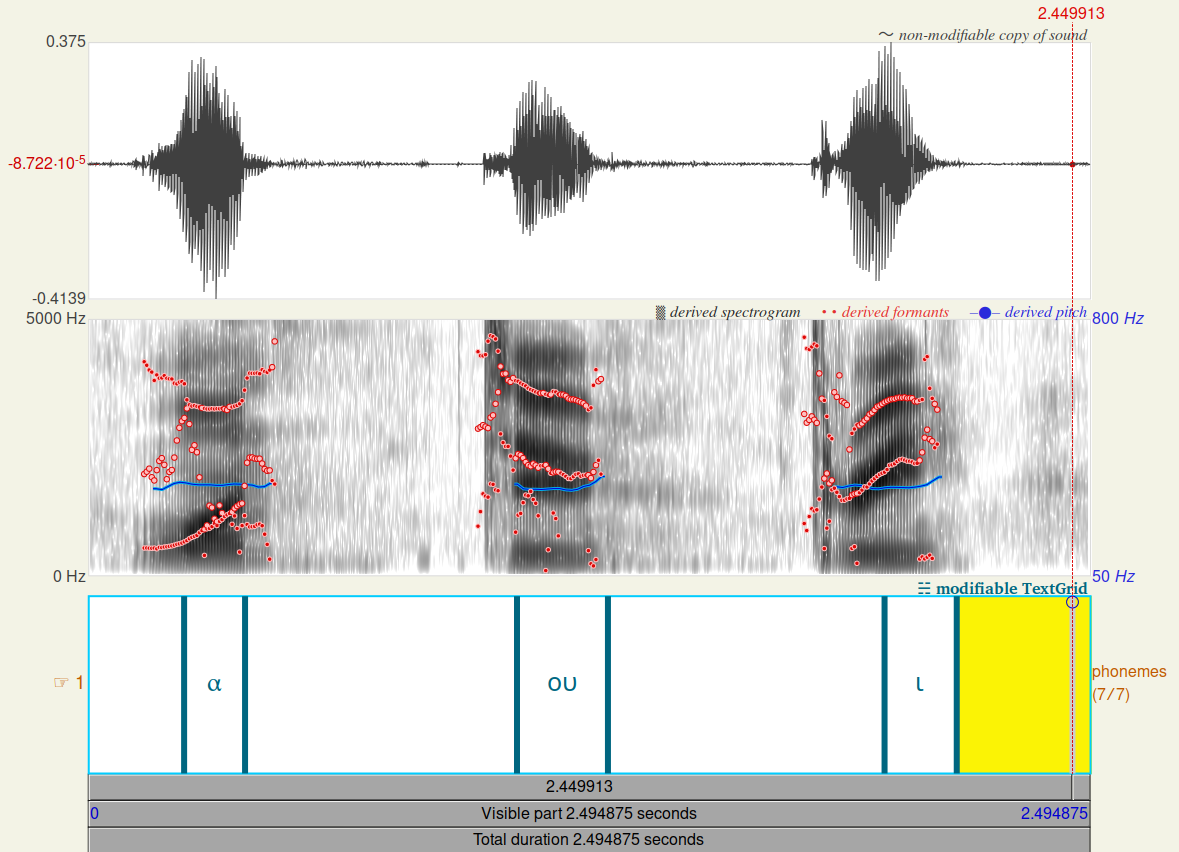
\includegraphics[width=0.6\linewidth]{plots/onetwothree1_praat.png}
\end{figure}

\noindent Τέλος σχεδιάσαμε τα παρακάτω διαγράμματα που οπτικοποιούν την εργασία μας (1ο) και τις μετρήσεις μας (2ο)

\begin{figure}[H]
	\centering
	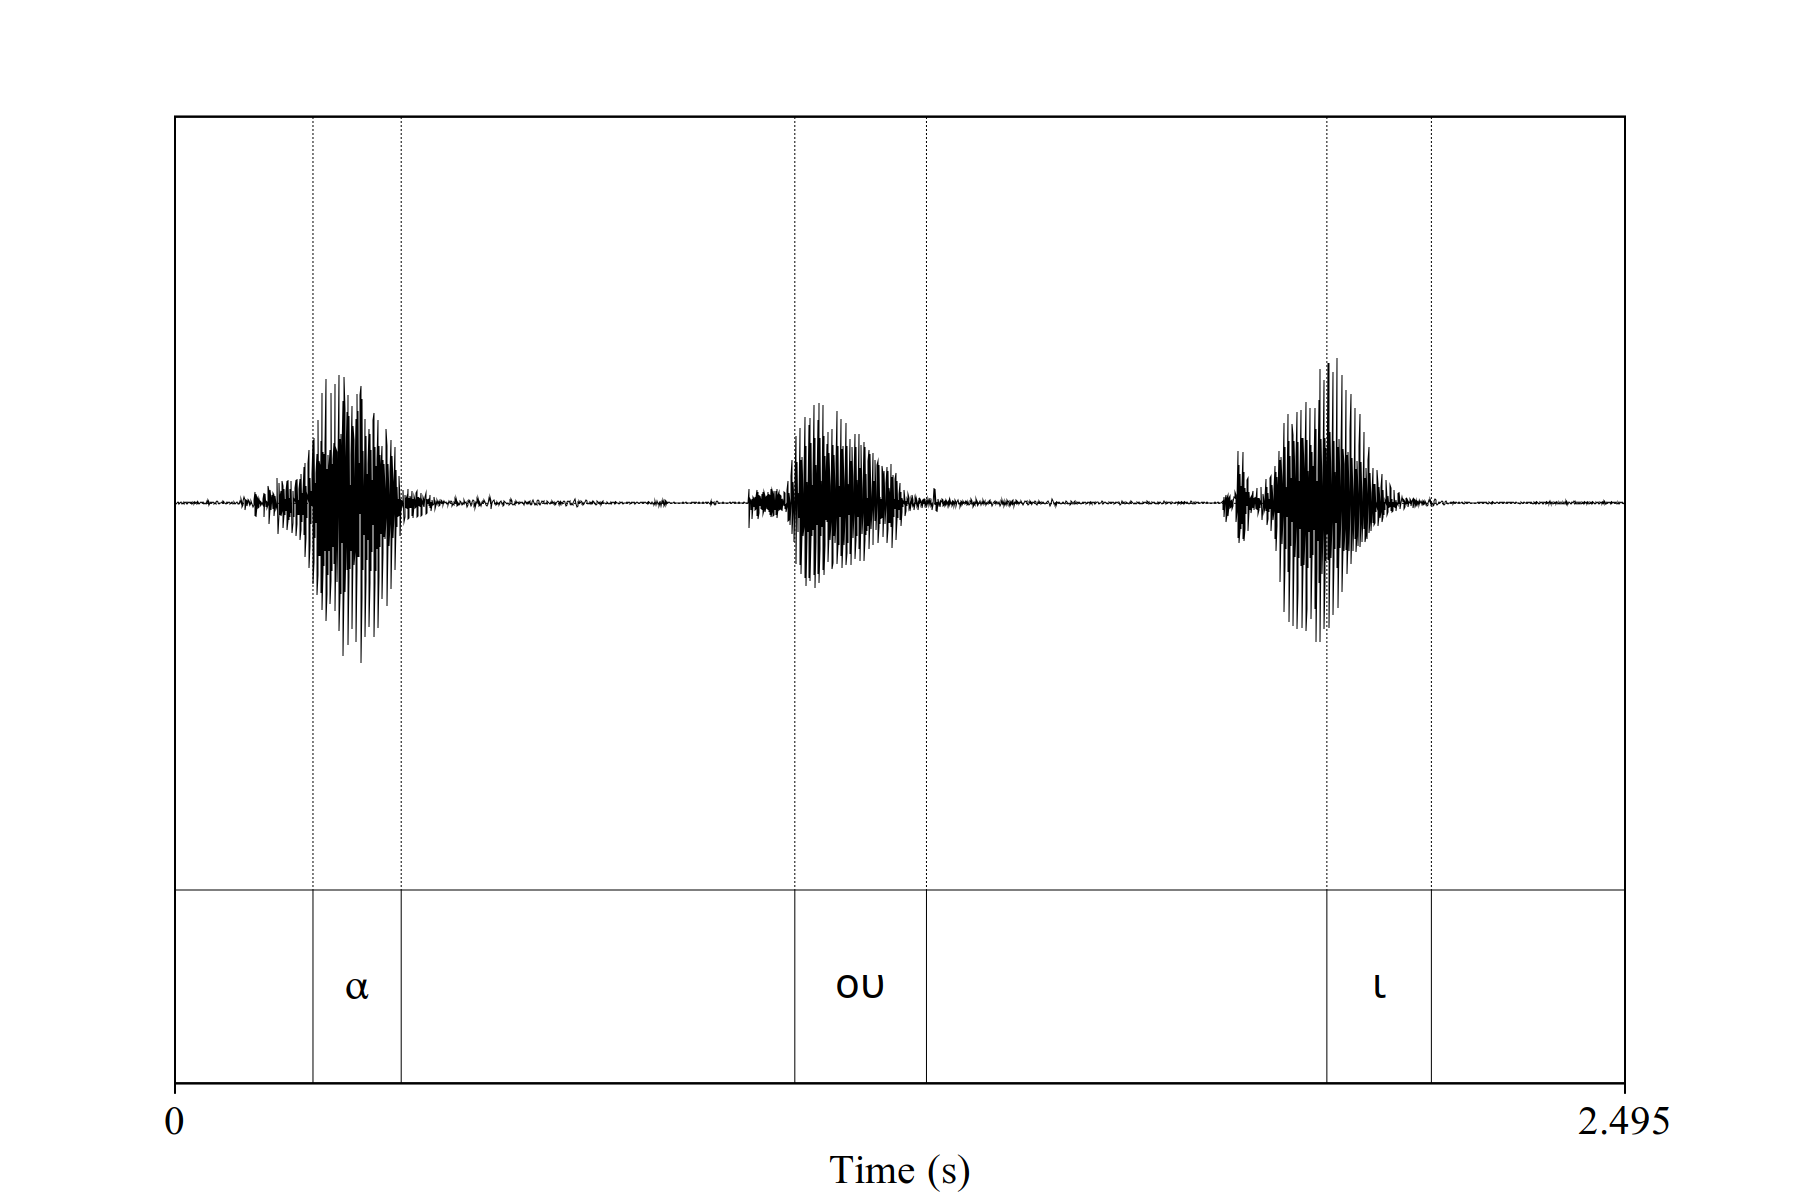
\includegraphics[width=0.6\linewidth]{plots/onetwothree1_annot.png}
\end{figure}

\begin{figure}[H]
	\centering
	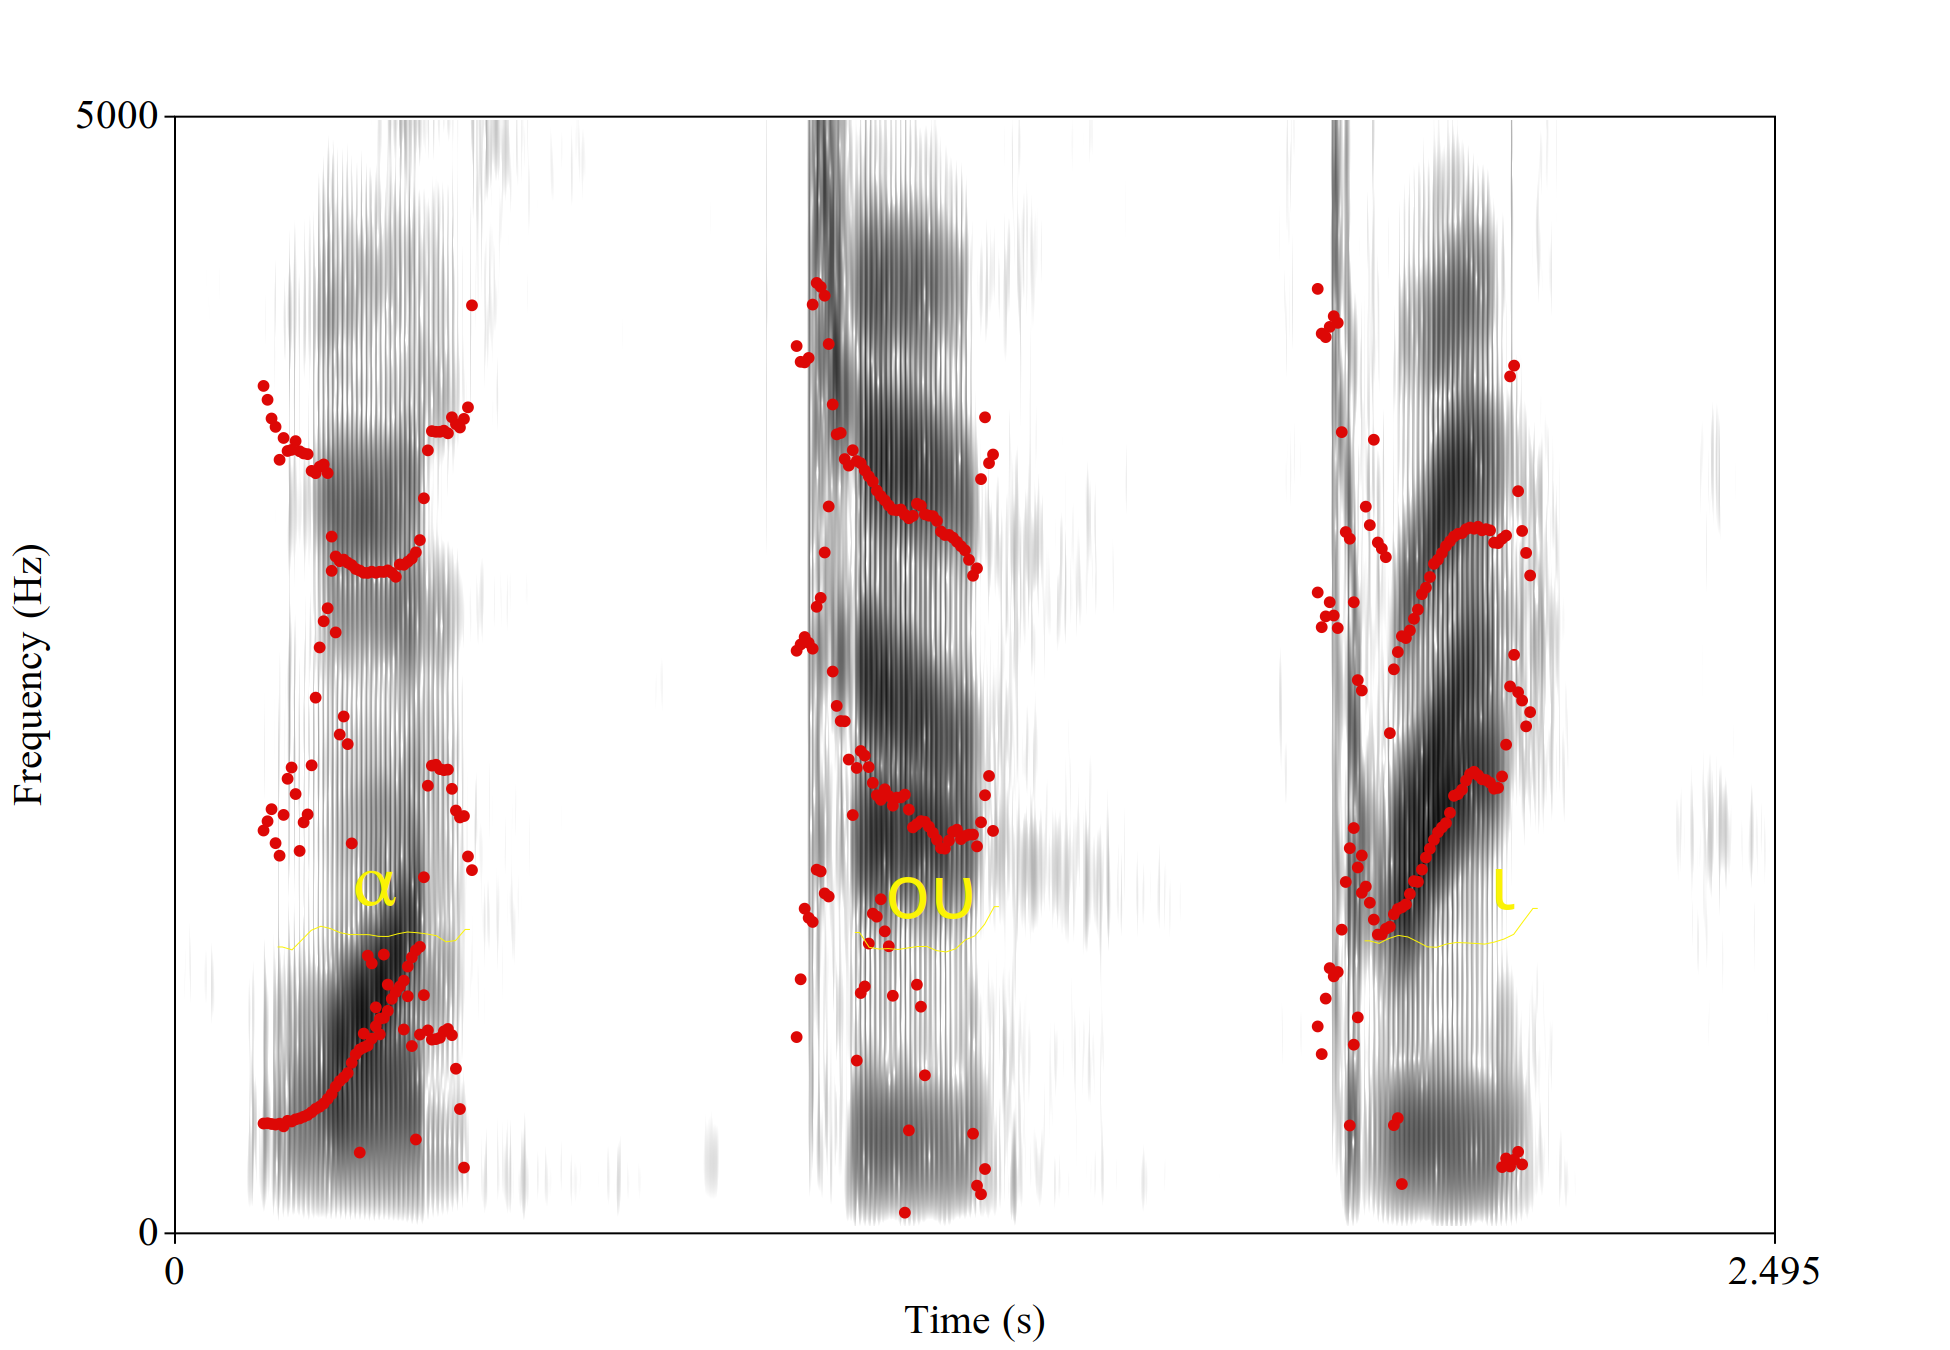
\includegraphics[width=0.7\linewidth]{plots/spectrogram_pitch_formants1.png}
\end{figure}

\subsection*{Αρχείο onetwothree8.wav}

Αντίστοιχα με το προηγούμενο αρχείο οι μετρήσεις μας για το pitch κάθε φωνήματος είναι:

\begin{itemize}
	\item \textbf{Pitch (α):} 178.90096253179337 Hz (mean pitch in SELECTION)
	\item \textbf{Pitch (ου):} 183.19462142657264 Hz (mean pitch in SELECTION)
	\item \textbf{Pitch (ι):} 176.88367983435367 Hz (mean pitch in SELECTION)
\end{itemize}

\noindent Για τα formants:

\begin{itemize}
	\item \textbf{Φώνημα α:}
	\begin{itemize}
		\item \textbf{F1\_Hz:} 674.367922
		\item \textbf{F2\_Hz:} 703.507187
		\item \textbf{F3\_Hz:} 4112.994619 
	\end{itemize}
	
	\item \textbf{Φώνημα ου:}
	\begin{itemize}
		\item \textbf{F1\_Hz:} 376.486131
		\item \textbf{F2\_Hz:} 2801.849314
		\item \textbf{F3\_Hz:} 3860.898207
	\end{itemize}
	
	\item \textbf{Φώνημα ι:}
	\begin{itemize}
		\item \textbf{F1\_Hz:} 345.351842 
		\item \textbf{F2\_Hz:} 2549.549245 
		\item \textbf{F3\_Hz:} 3396.739966
	\end{itemize}
\end{itemize}

\noindent Τα αντίστοιχα διαγράμματα είναι:

\begin{figure}[H]
	\centering
	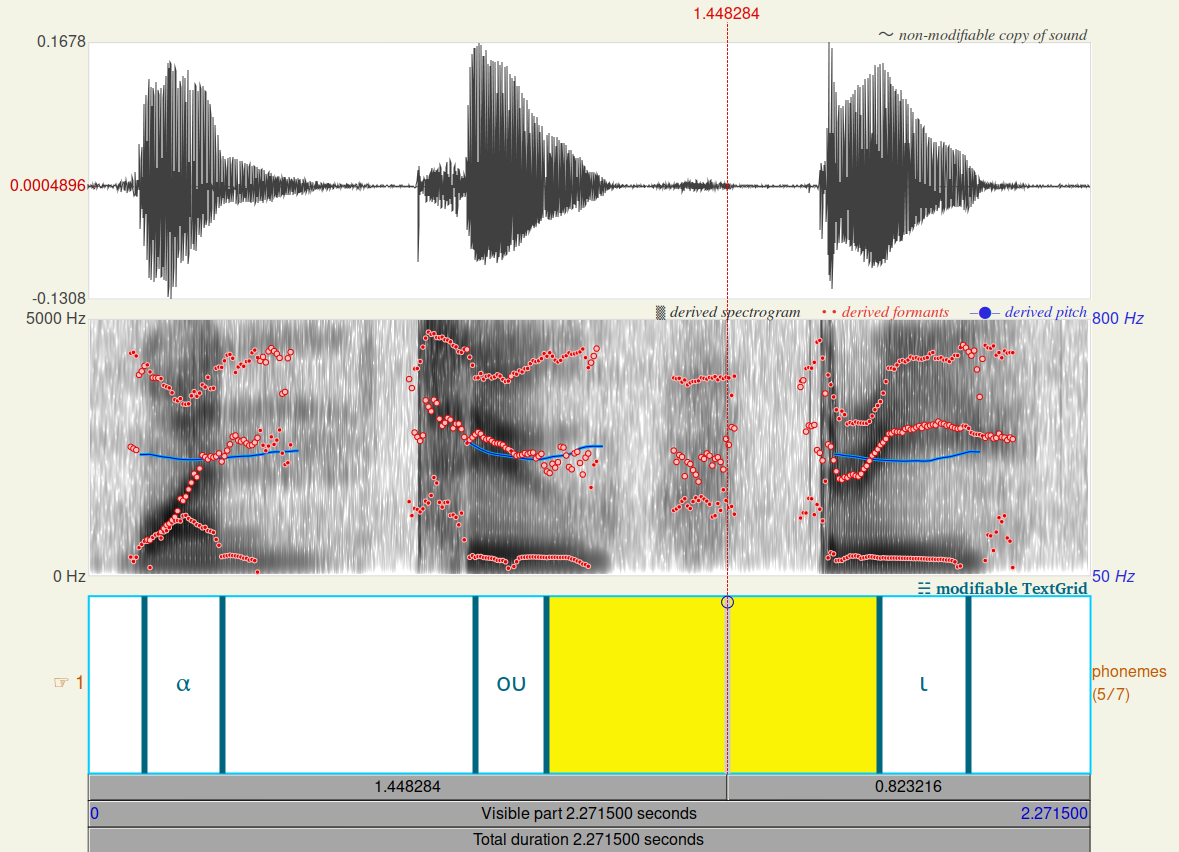
\includegraphics[width=0.5\linewidth]{plots/onetwothree8.png}
\end{figure}

\begin{figure}[H]
	\centering
	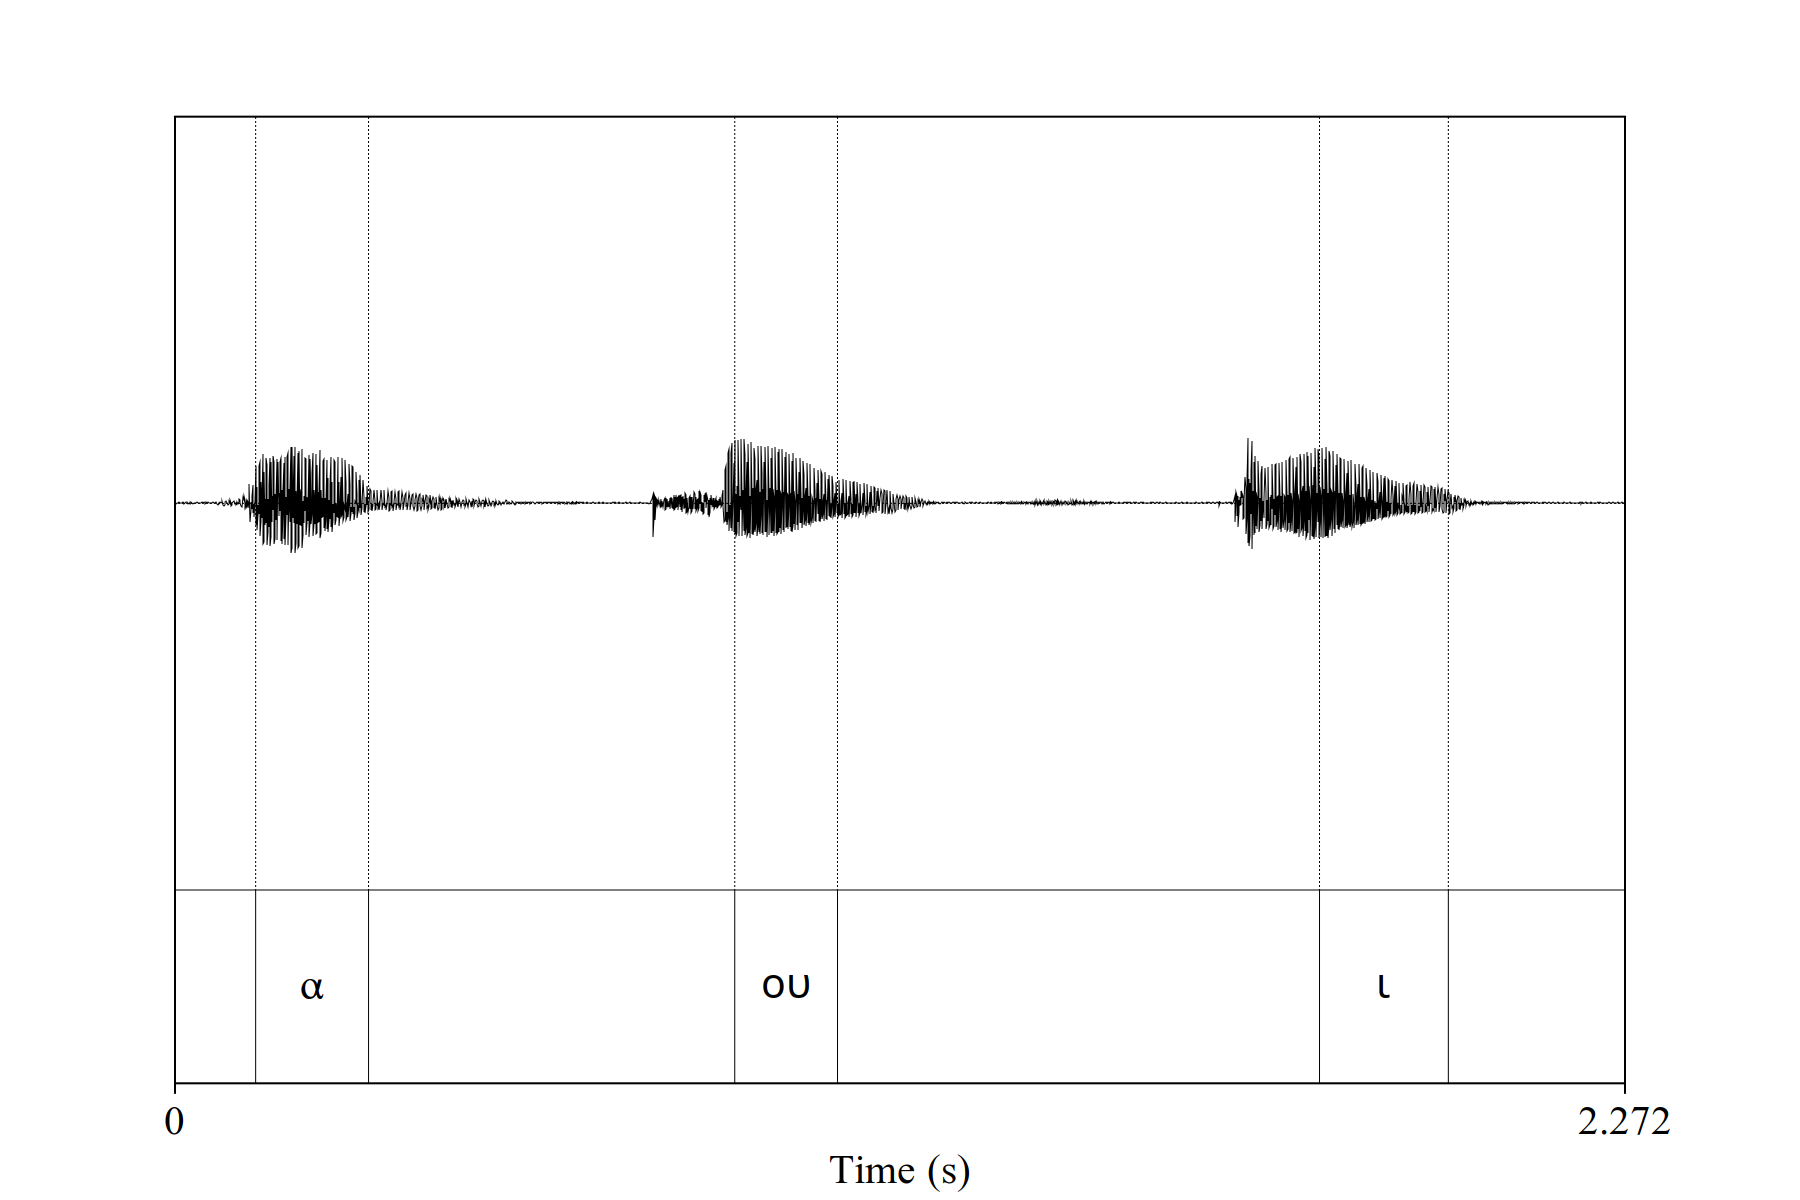
\includegraphics[width=0.55\linewidth]{plots/onetwothree8_annot.png}
\end{figure}

\begin{figure}[H]
	\centering
	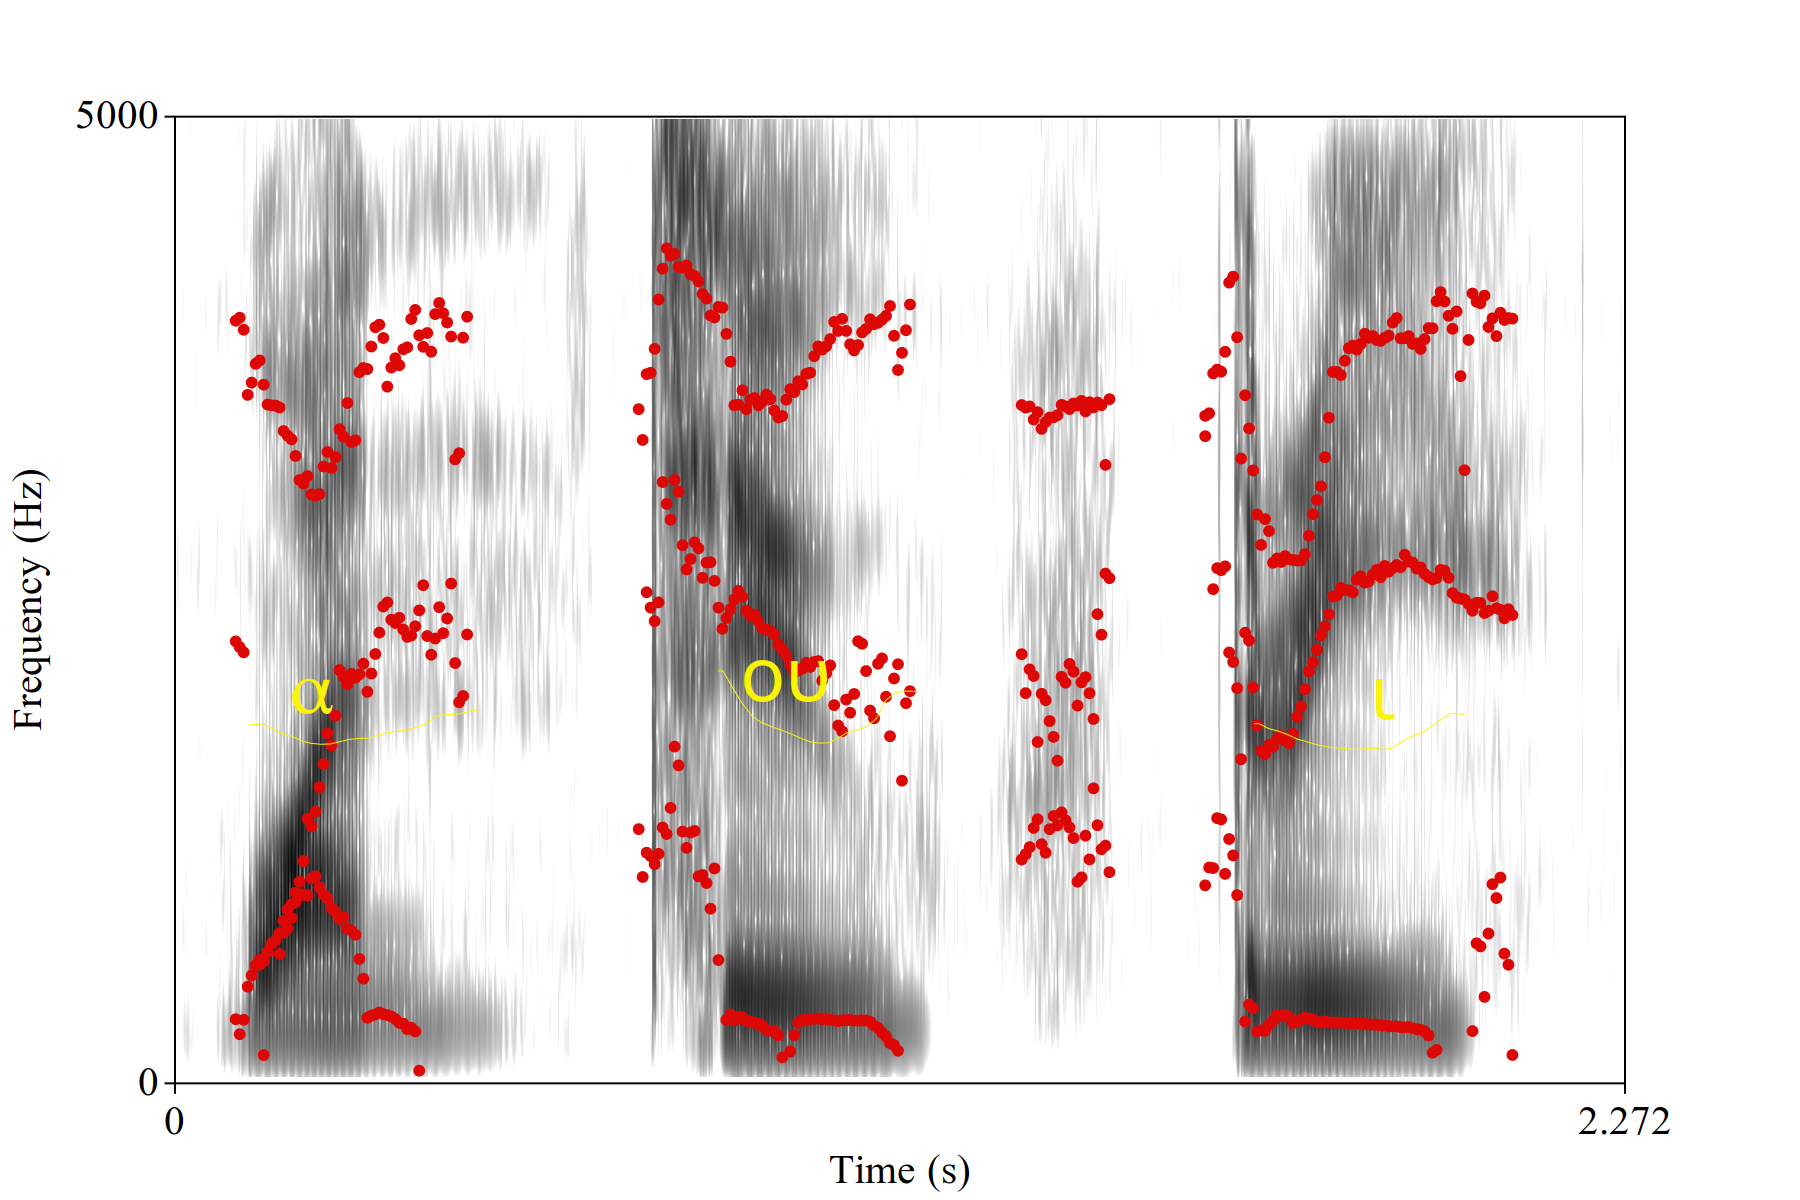
\includegraphics[width=0.55\linewidth]{plots/onetwothree8_info.png}
\end{figure}

\subsection*{Συμπεράσματα}
Βλέπουμε πως οι μετρήσεις μας συμφωνούν απόλυτα με τις θεωρητικές προσδοκίες που αναφέρθηκαν στην περιγραφή παραπάνω. Πιο συγκεκριμένα, τα pitch (μέσες τιμές) της γυναίκας (αρχείο onetwothree8.wav) βρίσκονται σε υψηλότερες συχνότητες από τις αντίστοιχες του άντρα. \\

\noindent Επιπλέον, κατά κανόνα τα formants του άντρα βρίσκονται σε χαμηλότερες συχνότητες αντανακλώντας τα διαφορετικά φυσικά χαρακτηριστικά της φωνητικής του οδού (είναι μεγαλύτερη).

\section*{Βήμα 2}

Στο βήμα αυτό ξεκινάει ο κώδικάς μας σε Python 3.

\noindent Ξεκινάμε γράφοντας την συνάρτηση data\_parser που σκανάρει τον φάκελο \verb|pr_lab2_data / digits| και επιστρέφει τρεις λίστες που περιέχουν τα δεδομένα των αρχείων wav, το id των ομιλητών και το ψηφίο που εκφωνούν, αντίστοιχα. 

\noindent Τα δεδομένα του αρχείου wav τα φορτώνουμε με τη συνάρτηση load της βιβλιοθήκης librosa, τα ids των ομιλητών με την μέθοδο isdigit() των strings, και τα ψηφία με την μέθοδο isalpha() στο τμήμα του filename πριν την κατάληξη.

\lstinputlisting[language=Python, firstline=26, lastline=44]{preparation.py}

\noindent Στην συνάρτηση main καλούμε την συνάρτηση data\_parser που μόλις γράψαμε ως εξής:

\lstinputlisting[language=Python, firstline=829, lastline=831]{preparation.py}

\noindent Στο τέλος, όπως φαίνεται στον κώδικα παραπάνω, κάνουμε μία ανάλυση των στατιστικών των ψηφίων.

\begin{figure}[H]
	\centering
	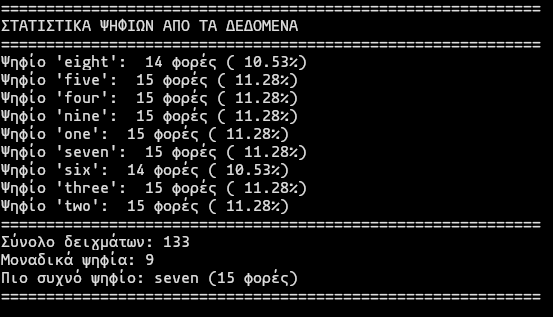
\includegraphics[width=0.55\linewidth]{plots/digits_stats.png}
\end{figure}

\noindent Αυτό το κάνουμε για να εξετάσουμε αν το dataset είναι ισορροπημένο ή όχι και αν όχι προς τα πού είναι biased. Όπως βλέπουμε, όμως, το dataset είναι ισορροπημένο. Έτσι, το accuracy θα είναι μία καλή μετρική για την αξιολόγηση των ταξινομητών που θα εκπαιδεύσουμε στη συνέχεια της εργασίας.

\section*{Βήμα 3}

Στο βήμα αυτό εξάγουμε τα Mel-frequency cepstral coefficients (MFCCs) των σημάτων. Οι συντελεστές αυτοί προκύπτουν από Discrete Cosine Transform εφαρμοσμένο στον λογάριθμο της φασματικής πυκνότητας ισχύος ειλημμένη στην κλίμακα mel ώστε ισαπέχοντα διαστήματα συχνοτήτων να ακούγονται εξίσου μακριά στο ανθρώπινο αυτί. Η διαφορά στην κλίμακα είναι που την διαφοροποιεί από το κανονικό cepstrum, του οποίο η διαδικασία παριστάνεται και γραφικά στο παρακάτω διάγραμμα του \cite{RabinerSchafer1978}.

\begin{figure}[H]
	\centering
	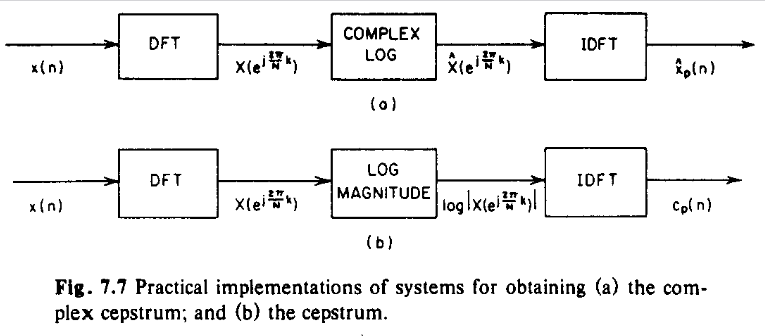
\includegraphics[width=0.7\linewidth]{plots/cepstrum.png}
\end{figure}

\noindent Χρησιμοποιούμε παράθυρο μήκους 25ms, βήμα 10ms και εξάγουμε ως χαρακτηριστικά τα 13 MFCCs ανά αρχείο. Επιπλέον, υπολογίζουμε την πρώτη και δεύτερη διακριτή παράγωγο των MFCCs κατά την μετακίνηση του παραθύρου λήψης τους. Η βιβλιοθήκη librosa έχει συναρτήσεις για όλα αυτά τα ζητούμενα, οπότε η τελική συνάρτηση και η κλήση της στη main φαίνονται παρακάτω:

\lstinputlisting[language=Python, firstline=73, lastline=87]{preparation.py}

\lstinputlisting[language=Python, firstline=833, lastline=834]{preparation.py}

\section*{Βήμα 4}

Αρχικά, δημιουργούμε ιστογράμματα για το 1ο και 2ο MFCC για όλες τις εκφωνήσεις των ψηφίων $n_1 = 2$ και $n_2 = 5$.

\begin{figure}[H]
	\centering
	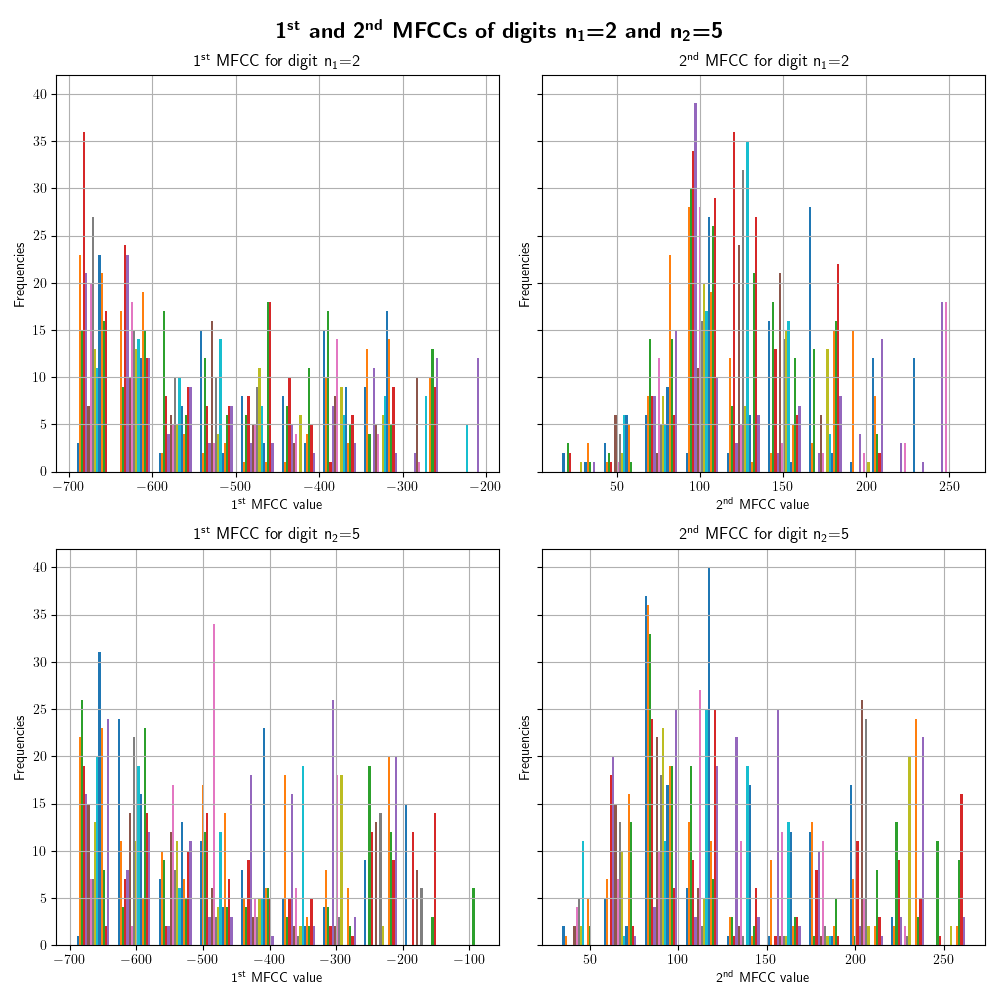
\includegraphics[width=\linewidth]{plots/histograms_step4.png}
\end{figure}

\noindent Αυτό που παρατηρούμε είναι ότι τα MFCC για $n_1=2$ δεν μοιάζουν πολύ μεταξύ τους στο ιστόγραμμα. Αυτό επιβεβαιώνεται και στο επόμενο γράφημα που αναπαριστά τη συσχέτιση μεταξύ τους, καθώς βλέπουμε ότι έχει τιμή 0,03 (γκρι χρώμα), για τον πρώτο ομιλητή. Από την άλλη πλευρά δεν παρατηρούμε το ίδιο για τον δεύτερο ομιλητή, πράγμα μη ευνοϊκό για το consistency της διαχωρισιμότητας των ψηφίων ανάμεσα στους ομιλητές. Αυτή τη παρατήρηση έρχονται να επιβεβαιώσουν και τα ιστογράμματα για $n_2=5$. Σε αυτά βλέπουμε ότι η μορφή τους μοιάζει αλλά και η συσχέτισή τους είναι υψηλή και για τους 2 ομιλητές (κοντά στο 0,85).

\noindent Επιπλέον, όσον αφορά την ικανότητα των MFCC να διαχωρίσουν τα διαφορετικά ψηφία, αυτό που μπορούμε να πούμε διαφάζοντας κατακόρυφα το διάγραμμα είναι ότι τα ιστογράμματα μοιάζουν μεν, δεν είναι πανομοιότυπα δε. Οπότε τα MFCC θα μπορούσαν να είναι η βάση του classification ειδικά εφόσον μετασχηματιστούν σε κάτι άλλο ή από αυτά εξαχθούν ορισμένα στατιστικά χαρακτηριστικά, πράγμα που κάνουμε παρακάτω με την μέση τιμή και την τυπική απόκλισή τους. 

\noindent Στη συνέχεια, υπολογίζουμε τα Mel Filterbank Spectral Coefficients (MFSCs) για δύο εκφωνήσεις των ίδιων ψηφίων από δύο διαφορετικούς ομιλητές και υπολογίζουμε τον πίνακα συνδιακύμανσης τους για κάθε εκφώνηση με την συνάρτηση corrcoef της numpy, παρουσιάζοντας το τελικό αποτέλεσμα σε heatmap της βιβλιοθήκης seaborn.

\begin{figure}[H]
	\centering
	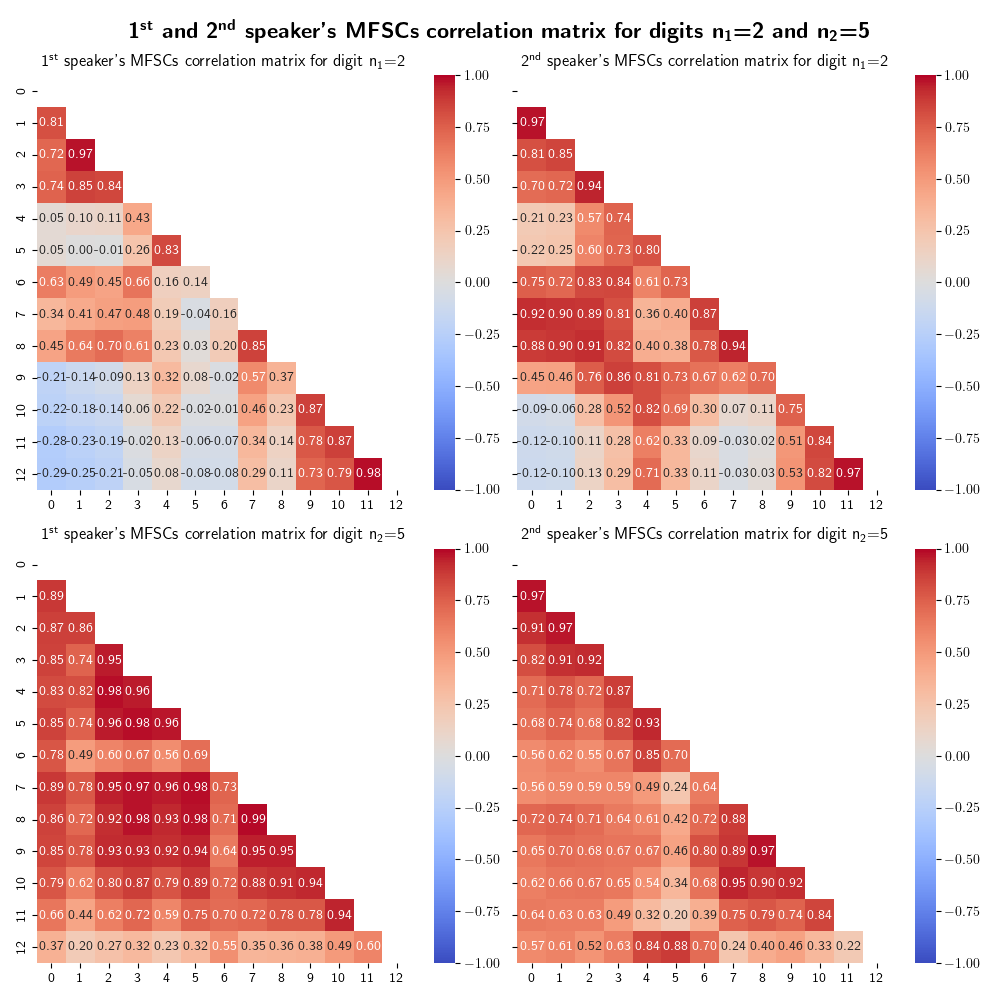
\includegraphics[width=\linewidth]{plots/corrs_mfsc_step4.png}
\end{figure}

\noindent Ύστερα, κάνουμε το ίδιο για τα MFCCs.

\begin{figure}[H]
	\centering
	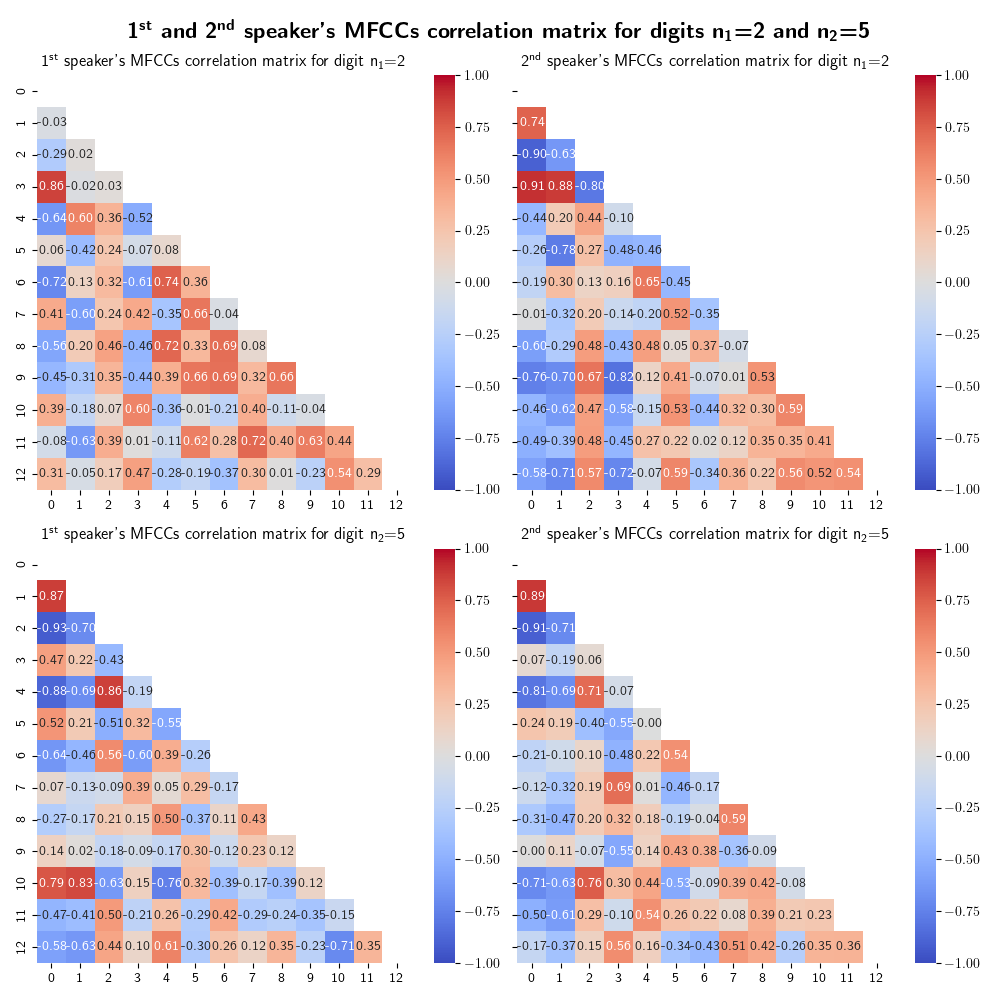
\includegraphics[width=\linewidth]{plots/corrs_mfcc_step4.png}
\end{figure}

\noindent Παρατηρούμε ότι τα MFCCs έχουν πολύ μικρότερη συσχέτιση μεταξύ τους. Για αυτόν τον λόγο, όταν κάνουμε επιλογή χαρακτηριστικών, χρησιμοποιούμε τα MFCCs αντί τα MFSCs, αφού στους περισσότερους αλγορίθμους προτιμάμε τα χαρακτηριστικά μας να είναι κατά το δυνατόν ανεξάρτητα, και το να είναι ασυσχέτιστα είναι προϋπόθεση για αυτό το γεγονός.\\

\noindent Σημειώνουμε ότι τα MSFCs τα λάβαμε με την εντολή \lstinline[language=Python]{librosa.feature.melspectrogram(y=wav, sr=Fs, win_length=win_len, hop_length=step, n_mels=n_features)}.
Ισοδύναμα, θα μπορούσαμε να τα είχαμε λάβει με την εντολή \lstinline[language=Python]{librosa.feature.inverse.mfcc_to_mel(mfcc)}, αφού η βιβλιοθήκη librosa έχει υλοποιημένη την μετατροπή MFCCs σε MFSCs,
ή με την εντολή \lstinline[language=Python]{librosa.db_to_power(scipy.fft.idct(mfcc, type=2, norm="ortho", axis=0))}, αφού τα MFSCs προκύπτουν με τον ίδιο ακριβώς τρόπο με τα MFCCs αλλά χωρίς την εφαρμογή του τελευταίου DFT, οπότε με Inverse DFS μπορούμε να τον αναιρέσουμε και να πάρουμε MFSCs από MFCCs. Την τριπλή αυτή ισοδυναμία επιβεβαιώσαμε και πειραματικά. Προτιμήσαμε τον πρώτο τρόπο, με το melspectrogram εφαρμοσμένο στο wav, γιατί εφαρμόζει τον ευθύ μετασχηματισμό, οπότε δεν υποφέρει από τα επιπλέον αριθμητικά σφάλματα που εισάγουν οι DCT και Inverse DCT.

\section*{Βήμα 5}
Αρχικά χρησιμοποιούμε NumPy για να ενώσουμε όλα τα χαρακτηριστικά του input που έχουμε υπολογίσει (mfcc, delta, delta-deltas) και να φτιάξουμε έναν πίνακα. Κατόπιν υπολογίζουμε για καθένα από αυτά τη μέση τιμή και την τυπική απόκλιση και επιλέγουμε αυτά ως τα τελικά χαρακτηριστικά που θα χρησιμοποιήσουμε για το classification. Στα σχόλια έχουμε το shape των tensors που έχουμε εκτυπώσει για να είμαστε σίγουροι για την ορθότητα των βημάτων μας.

\lstinputlisting[language=Python, firstline=211, lastline=223]{preparation.py}

\noindent Οι 2 πρώτες διαστάσεις που καλούμαστε να παραστήσουμε σε scatter plot είναι οι μέσες τιμές των πρώτων 2 MFCC. To αποτέλεσμα φαίνεται παρακάτω (ο λόγος που χρησιμοποιούμε διαφορετικά χρώματα και σχήματα είναι για να κάνουμε τις κλάσεις μας ευδιάκριτες):

\begin{figure}[H]
	\centering
	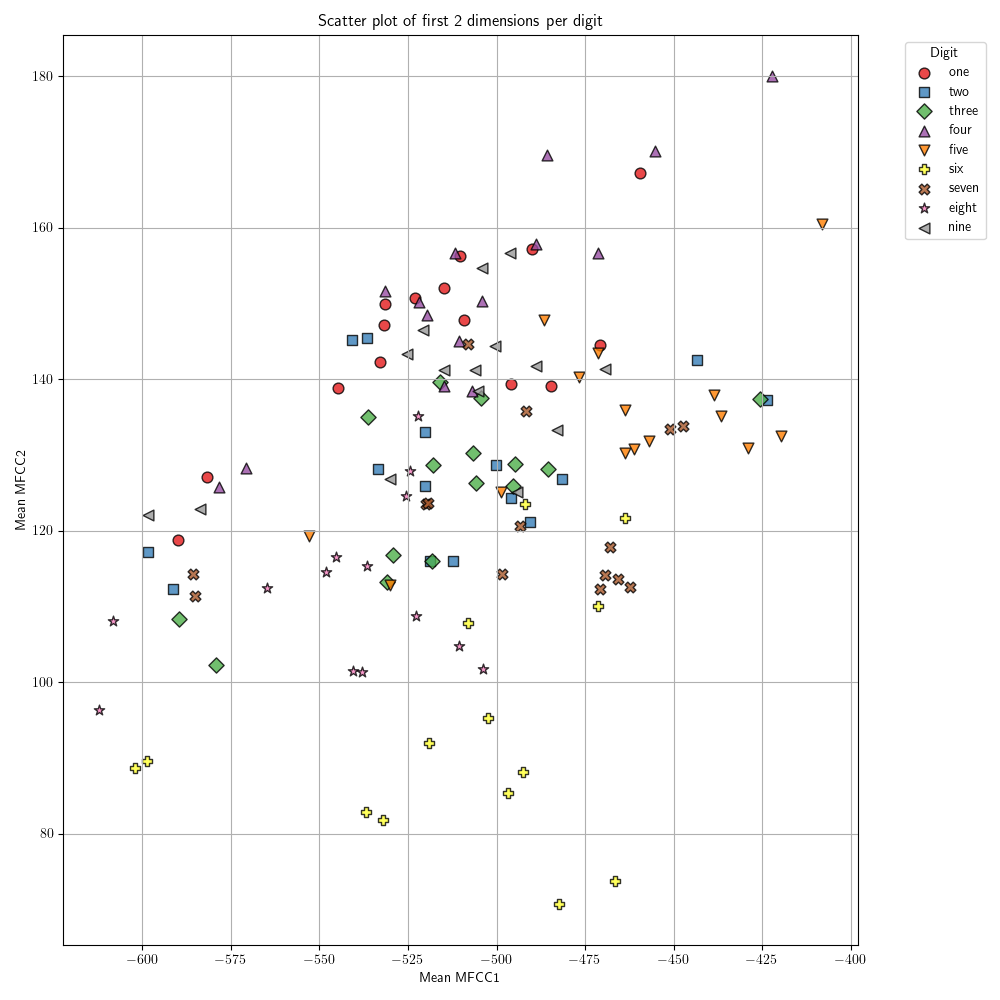
\includegraphics[width=\linewidth]{plots/scatter_plot_2_random_features_step5.png}
\end{figure}

\noindent Ουσιαστικά, αυτό που κάνουμε είναι να βάζουμε 2 "τυχαία" (έστω τα 2 πρώτα) features στο scatter plot για να δούμε ότι οι κλάσεις μας δεν είναι τόσο διαχωρίσιμες. Προετοιμαζόμαστε να συγκρίνουμε το αποτέλεσμα με το PCA στο βήμα 6 όπου τα 2 πρώτα features γίνονται εκείνα που εξηγούν το μεγαλύτερο ποσοστό του variance και έτσι κάνουν τις κλάσεις μας πιο διαχωρίσιμες από αυτό που βλέπουμε παραπάνω.

\section*{Βήμα 6}

Στο βήμα αυτό, εφαρμόζουμε Principal Component Analysis (PCA) για την μείωση διαστατικότητας των δεδομένων. Αρχικά, μειώνουμε τις διαστάεις των διανυσμάτων χαρακτηριστικών σε 2 με την εντολή \lstinline[language=Python]{PCA(n_components=2).fit_transform(feature_vectors)} και στη συνέχεια σε 3 θέτοντας n\_components = 3.\\

\noindent Παρακάτω παραθέτουμε εκ νέου το scatter plot με τις δύο διαστάσεις των μετασχηματισμένων δεδομένων για n\_components = 2.

\begin{figure}[H]
	\centering
	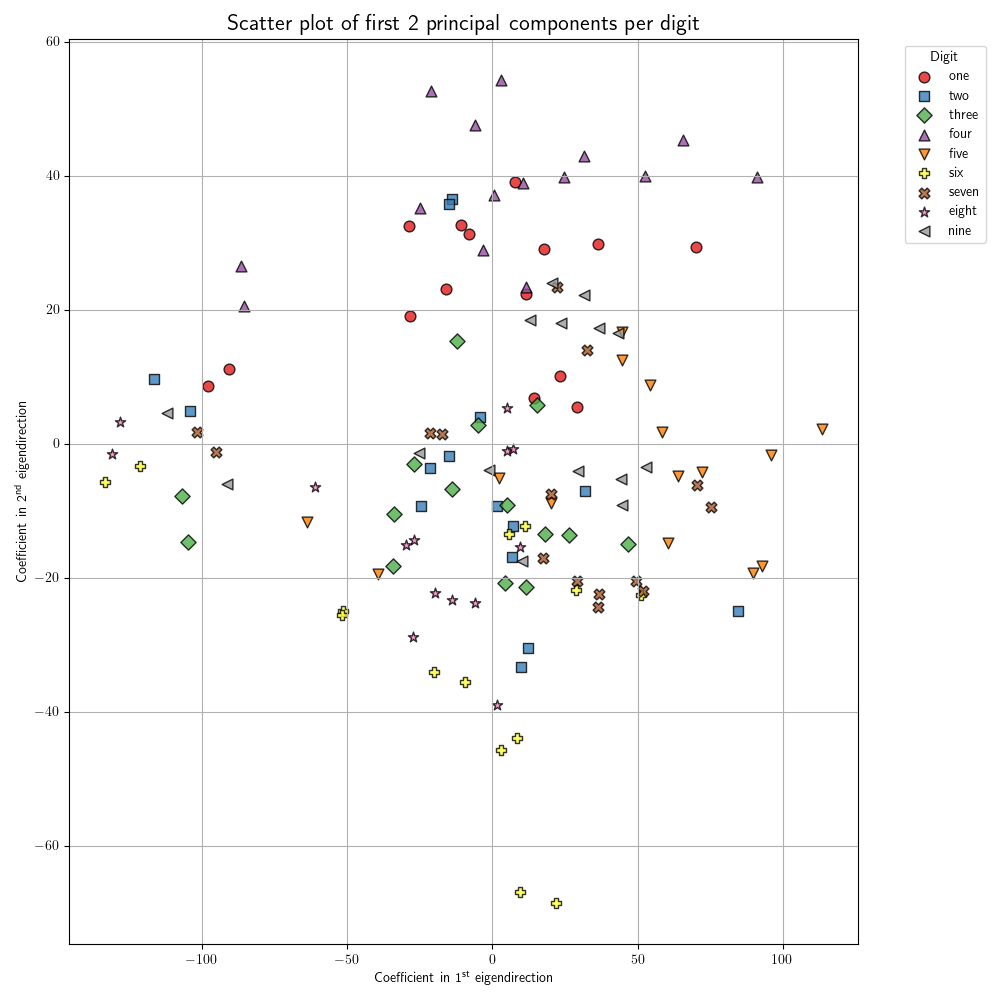
\includegraphics[width=\linewidth]{plots/scatter_plot_2_eigendirections_step6.png}
\end{figure}

\noindent Παρατηρούμε ότι τα σημεία ακόμα δεν είναι ιδιαίτερα διαχωρισμένα, αλλά πολύ περισσότερο από ό,τι στο Βήμα 5 χωρίς PCA. Τα ψηφία είναι καλύτερα μαζεμένα σε περιοχές, αλλά υπάρχουν πολλές επικαλύψεις ακόμα. Το ποσοστό της συνολικής ερμηνευόμενης διασποράς των δεδομένων είναι 70.5\% (άθροισμα στοιχείων πεδίου explained\_variance\_ratio\_).\\

\noindent Ακολούθως, παραθέτουμε το scatter plot με τις τρεις διαστάσεις των μετασχηματισμένων δεδομένων για n\_components = 3.

\begin{figure}[H]
	\centering
	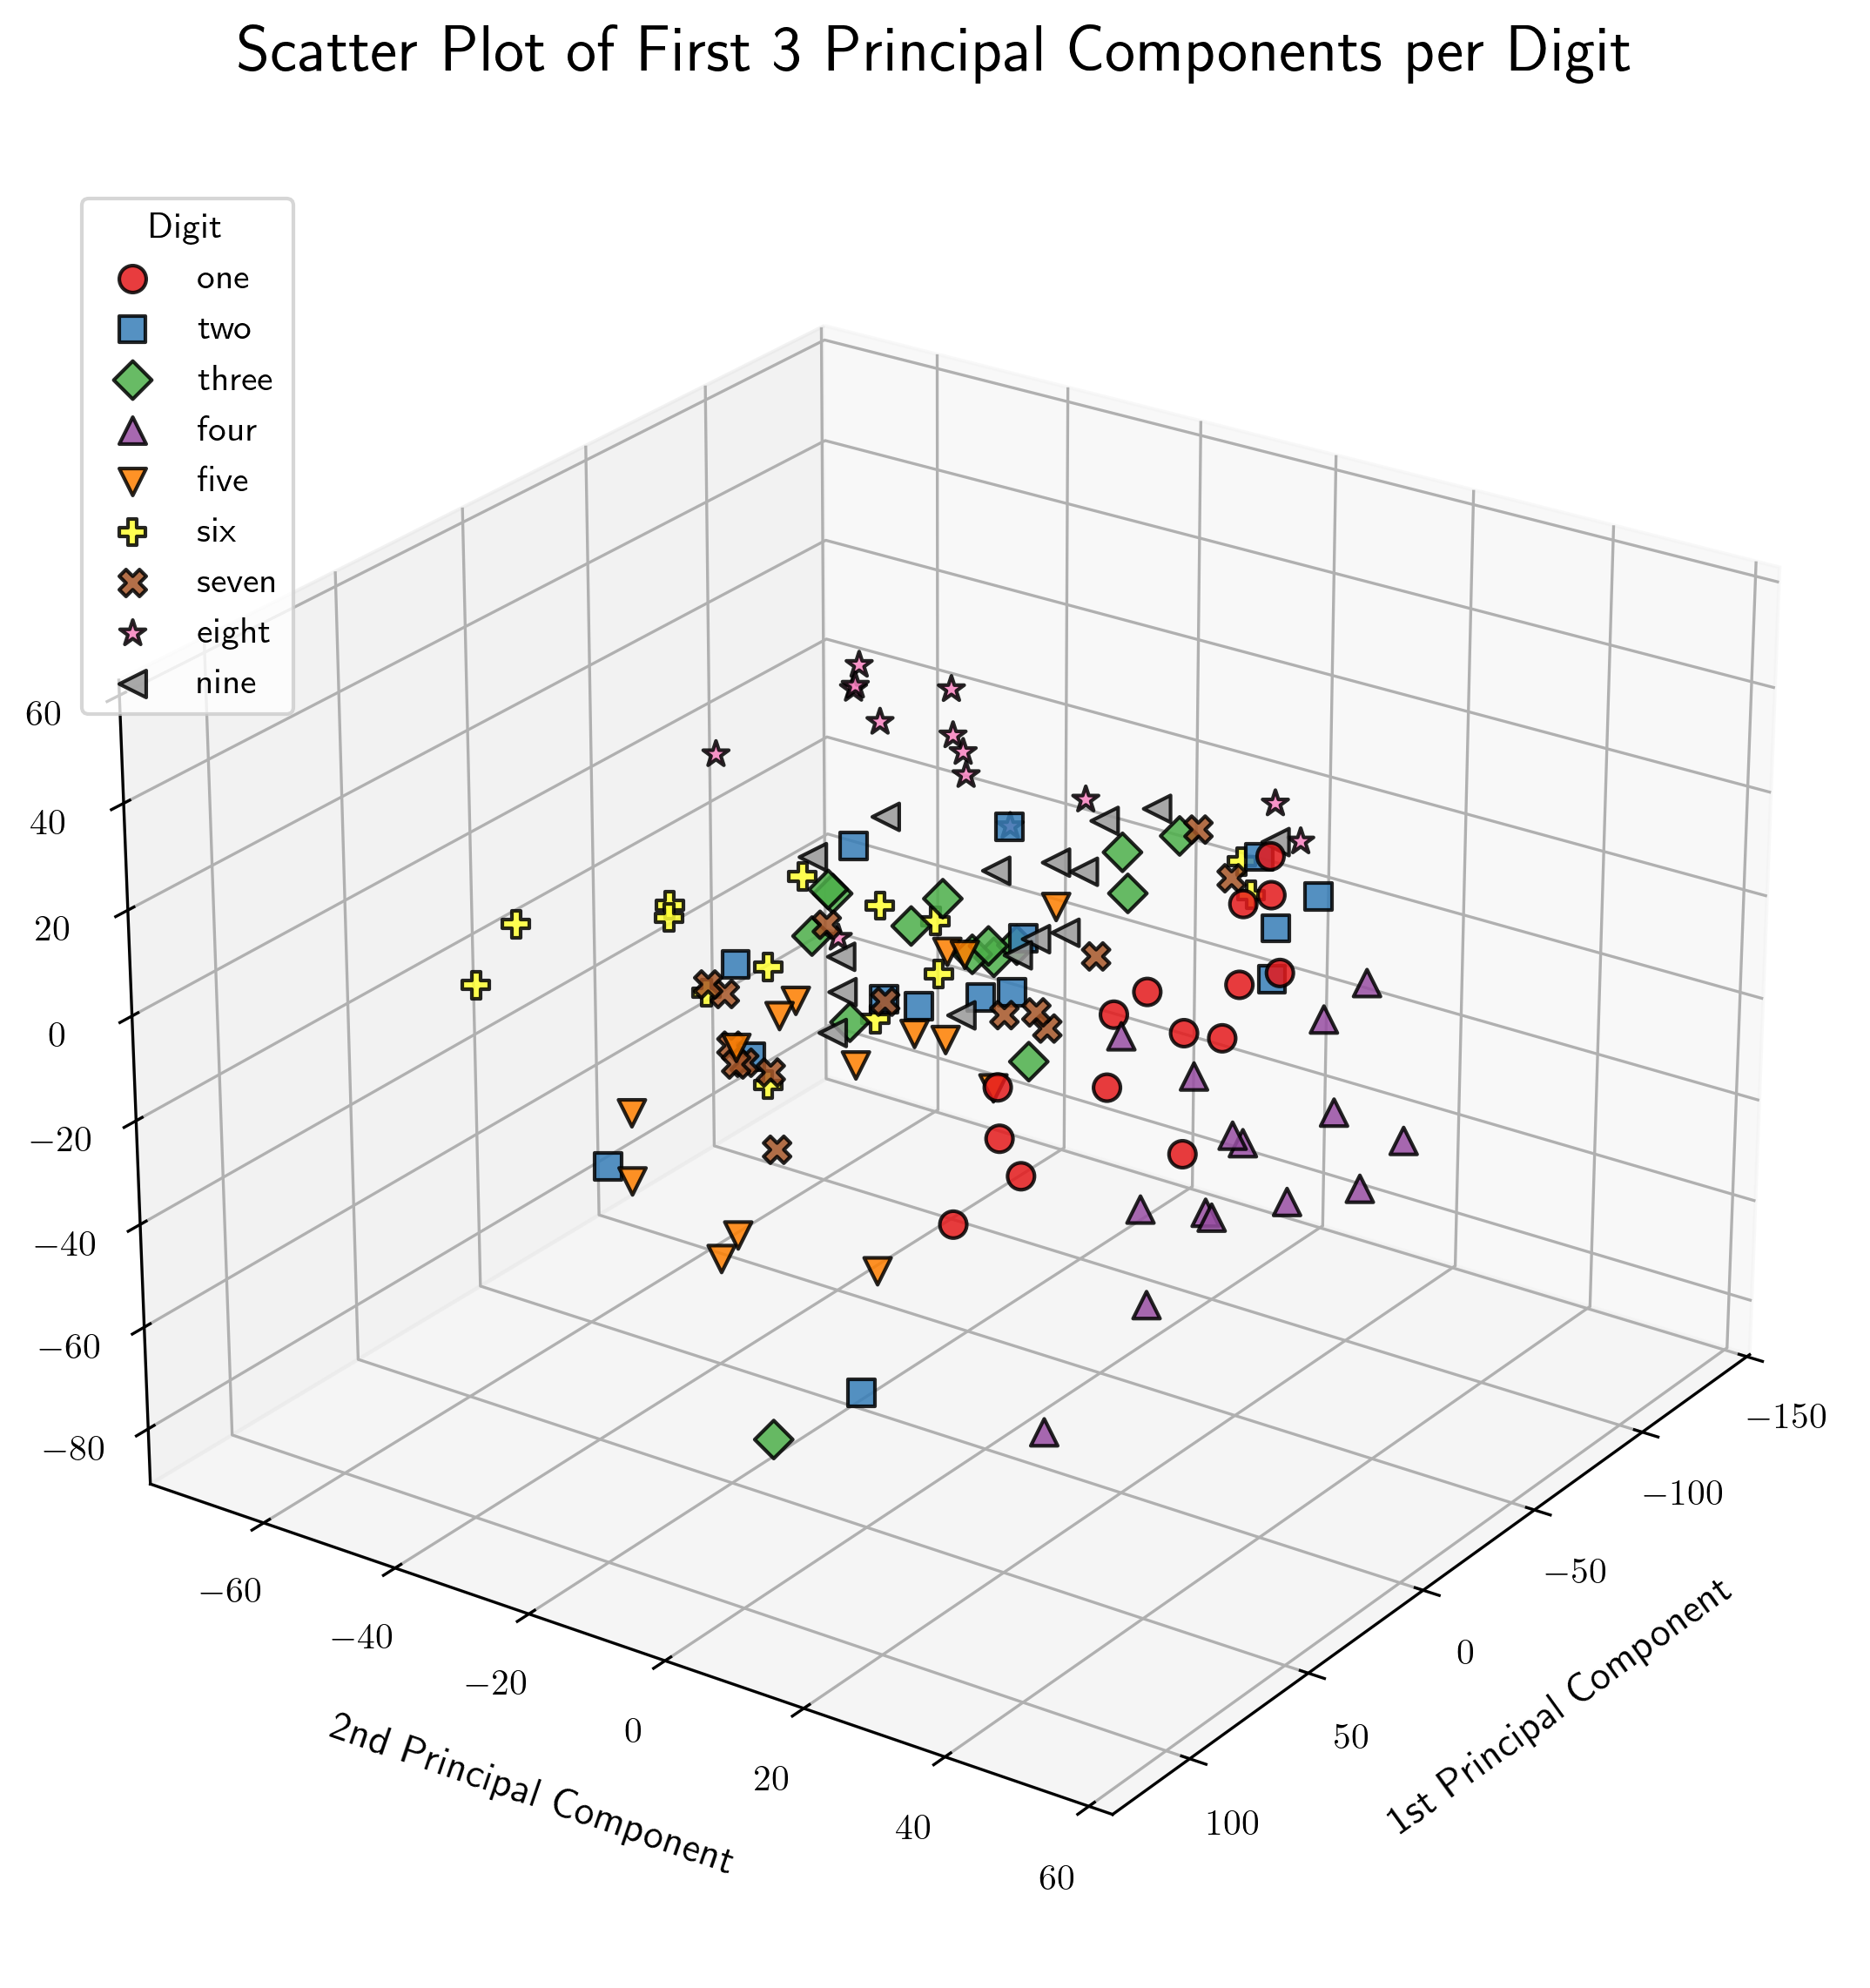
\includegraphics[width=\linewidth]{plots/scatter_plot_3_eigendirections_step6.png}
\end{figure}

\noindent Πλέον, παρατηρούμε ότι τα ψηφία είναι πολύ καλύτερα διαχωρισμένα. Είναι μαζεμένα σε συμπαγείς περιοχές και υπάρχουν πολύ λιγότερες επικαλύψεις, αν και ακόμα υπάρχουν. Επιπλέον, η συνολική ερμηνευόμενη διασπορά είναι 81.4\%. Ακόμα, το πεδίο explained\_variance\_ratio\_ μας δίνει το ποσοστό της ερμηνευόμενης διασποράς από κάθε συνιστώσα του PCA, δηλαδή τη διασπορά σε στον κάθε άξονα των πρώτων ιδιοδιανυσμάτων του πίνακα συνδιασποράς. Αυτή είναι πολύ μεγάλη για το πρώτο διάνυσμα και μονότονα μειώνεται όσο αυξάνονται οι συνιστώσες.\\

\noindent Μπορούμε να θεωρήσουμε ότι η μείωση διαστατικότητας ήταν επιτυχημένη, αφού ερμηνεύσαμε το 70.5\% και 81.4\% με μόνο 2 και 3 συνιστώσες αντίστοιχα, αλλά για να έχουμε ακόμα καλύτερη απόδοση, θα βοηθούσε να έχουμε λίγες ακόμα συνιστώσες ώστε να ερμηνεύσουμε ακόμα μεγαλύτερο τμήμα της διασποράς και να διαχωριστούν πλήρως τα δεδομένα.

\section*{Βήμα 7}

Στο βήμα αυτό, αρχικά χωρίζουμε τα δεδομένα μας σε δεδομένα εκπαίδευσης (train, 70\%) και δεδομένα ελέγχου (test, 30\%) με χρήση της συνάρτησης train\_test\_split. Προτού δοκιμάσουμε οποιοδήποτε μοντέλο κανονικοποιούμε τα δεδομένα για να τα χειρίζονται "δίκαια" μέθοδοι επιλογής χαρακτηριστικών όπως η PCA (που χρησιμοποιούμε ξανά) και μοντέλα ταξινόμησης που βασίζονται σε μετρικούς χώρους.\\

\noindent Ακολούθως, σε όλα τα μοντέλα μας θα δοκιμάζουμε ως υπερπαράμετρο το πλήθος συνιστωσών του PCA, από 2 έως και 10. Όλα τα μοντέλα θα αξιολογούνται στο τέλος με βάση το accuracy και το F1-score. Το F1-score το χρησιμοποιούμε κυρίως σε περιπτώσεις που υπάρχουν ανισορροπίες στην εκπροσώπηση των κλάσεων στα δεδομένα, κάτι που παρατηρούμε ότι εδώ δεν συμβαίνει. Για αυτό, σε όλα τα μοντέλα που εξετάζουμε, το accuracy και το f1-score είναι πολύ κοντά και έχουν την ίδια τάση.\\

\noindent Το πρώτο μοντέλο που δοκιμάζουμε είναι ο Naive Bayes για Γκαουσιανές τυχαίες μεταβλητές (\lstinline[language=Python]{GaussianNB()}). Παραθέτουμε το διάγραμμα των μετρικών ως προς το πλήθος συνιστωσών κατά το PCA. Το καλύτερο μοντέλο λήφθηκε για 10 συνιστώσες με ακρίβεια 60\%.

\begin{figure}[H]
	\centering
	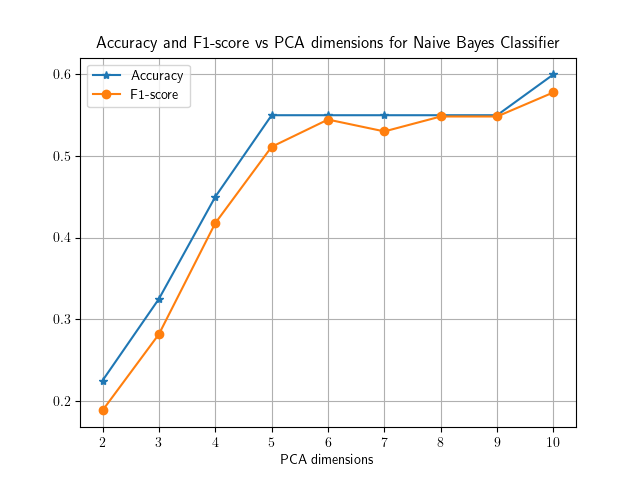
\includegraphics[width=\linewidth]{plots/accuracies_and_f1_naive_bayes_step7.png}
\end{figure}

\noindent Το δεύτερο μοντέλο που δοκιμάζουμε είναι το Support Vector Machine με το μη γραμμικό απειροδιάστατο RBF kernel (\lstinline[language=Python]{SVC()}). Παραθέτουμε και εδώ το αντίστοιχο διάγραμμα. Το καλύτερο μοντέλο λήγθηκε πάλι για 10 συνιστώσες με ακρίβεια 60\%.

\begin{figure}[H]
	\centering
	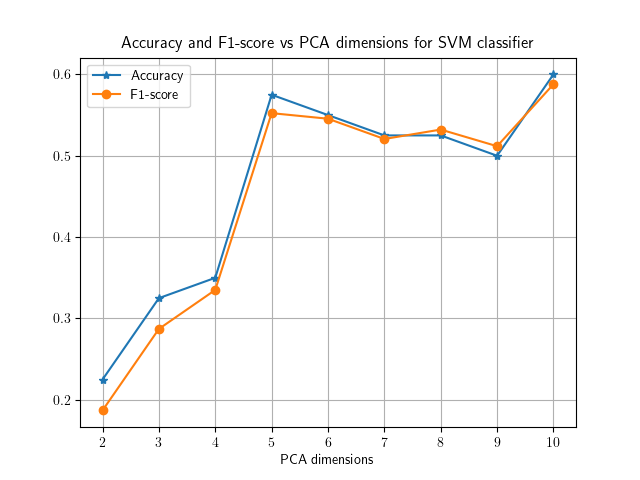
\includegraphics[width=\linewidth]{plots/accuracies_and_f1_svm_step7.png}
\end{figure}

\noindent Το τρίτο μοντέλο που δοκιμάζουμε είναι το k-Nearest Neigbors, με επιπλέον υπερπαράμετρο το $k \in \{1, 3, 5, 7\}$ (\lstinline[language=Python]{KNeighborsClassifier(n_neighbors=k)}). Παραθέτουμε το αντίστοιχο τριδιάστατο διάγραμμα. Το καλύτερο μοντέλο λήφθηκε για 10 συνιστώσες και k = 5 με ακρίβεια 70\%.

\begin{figure}[H]
	\centering
	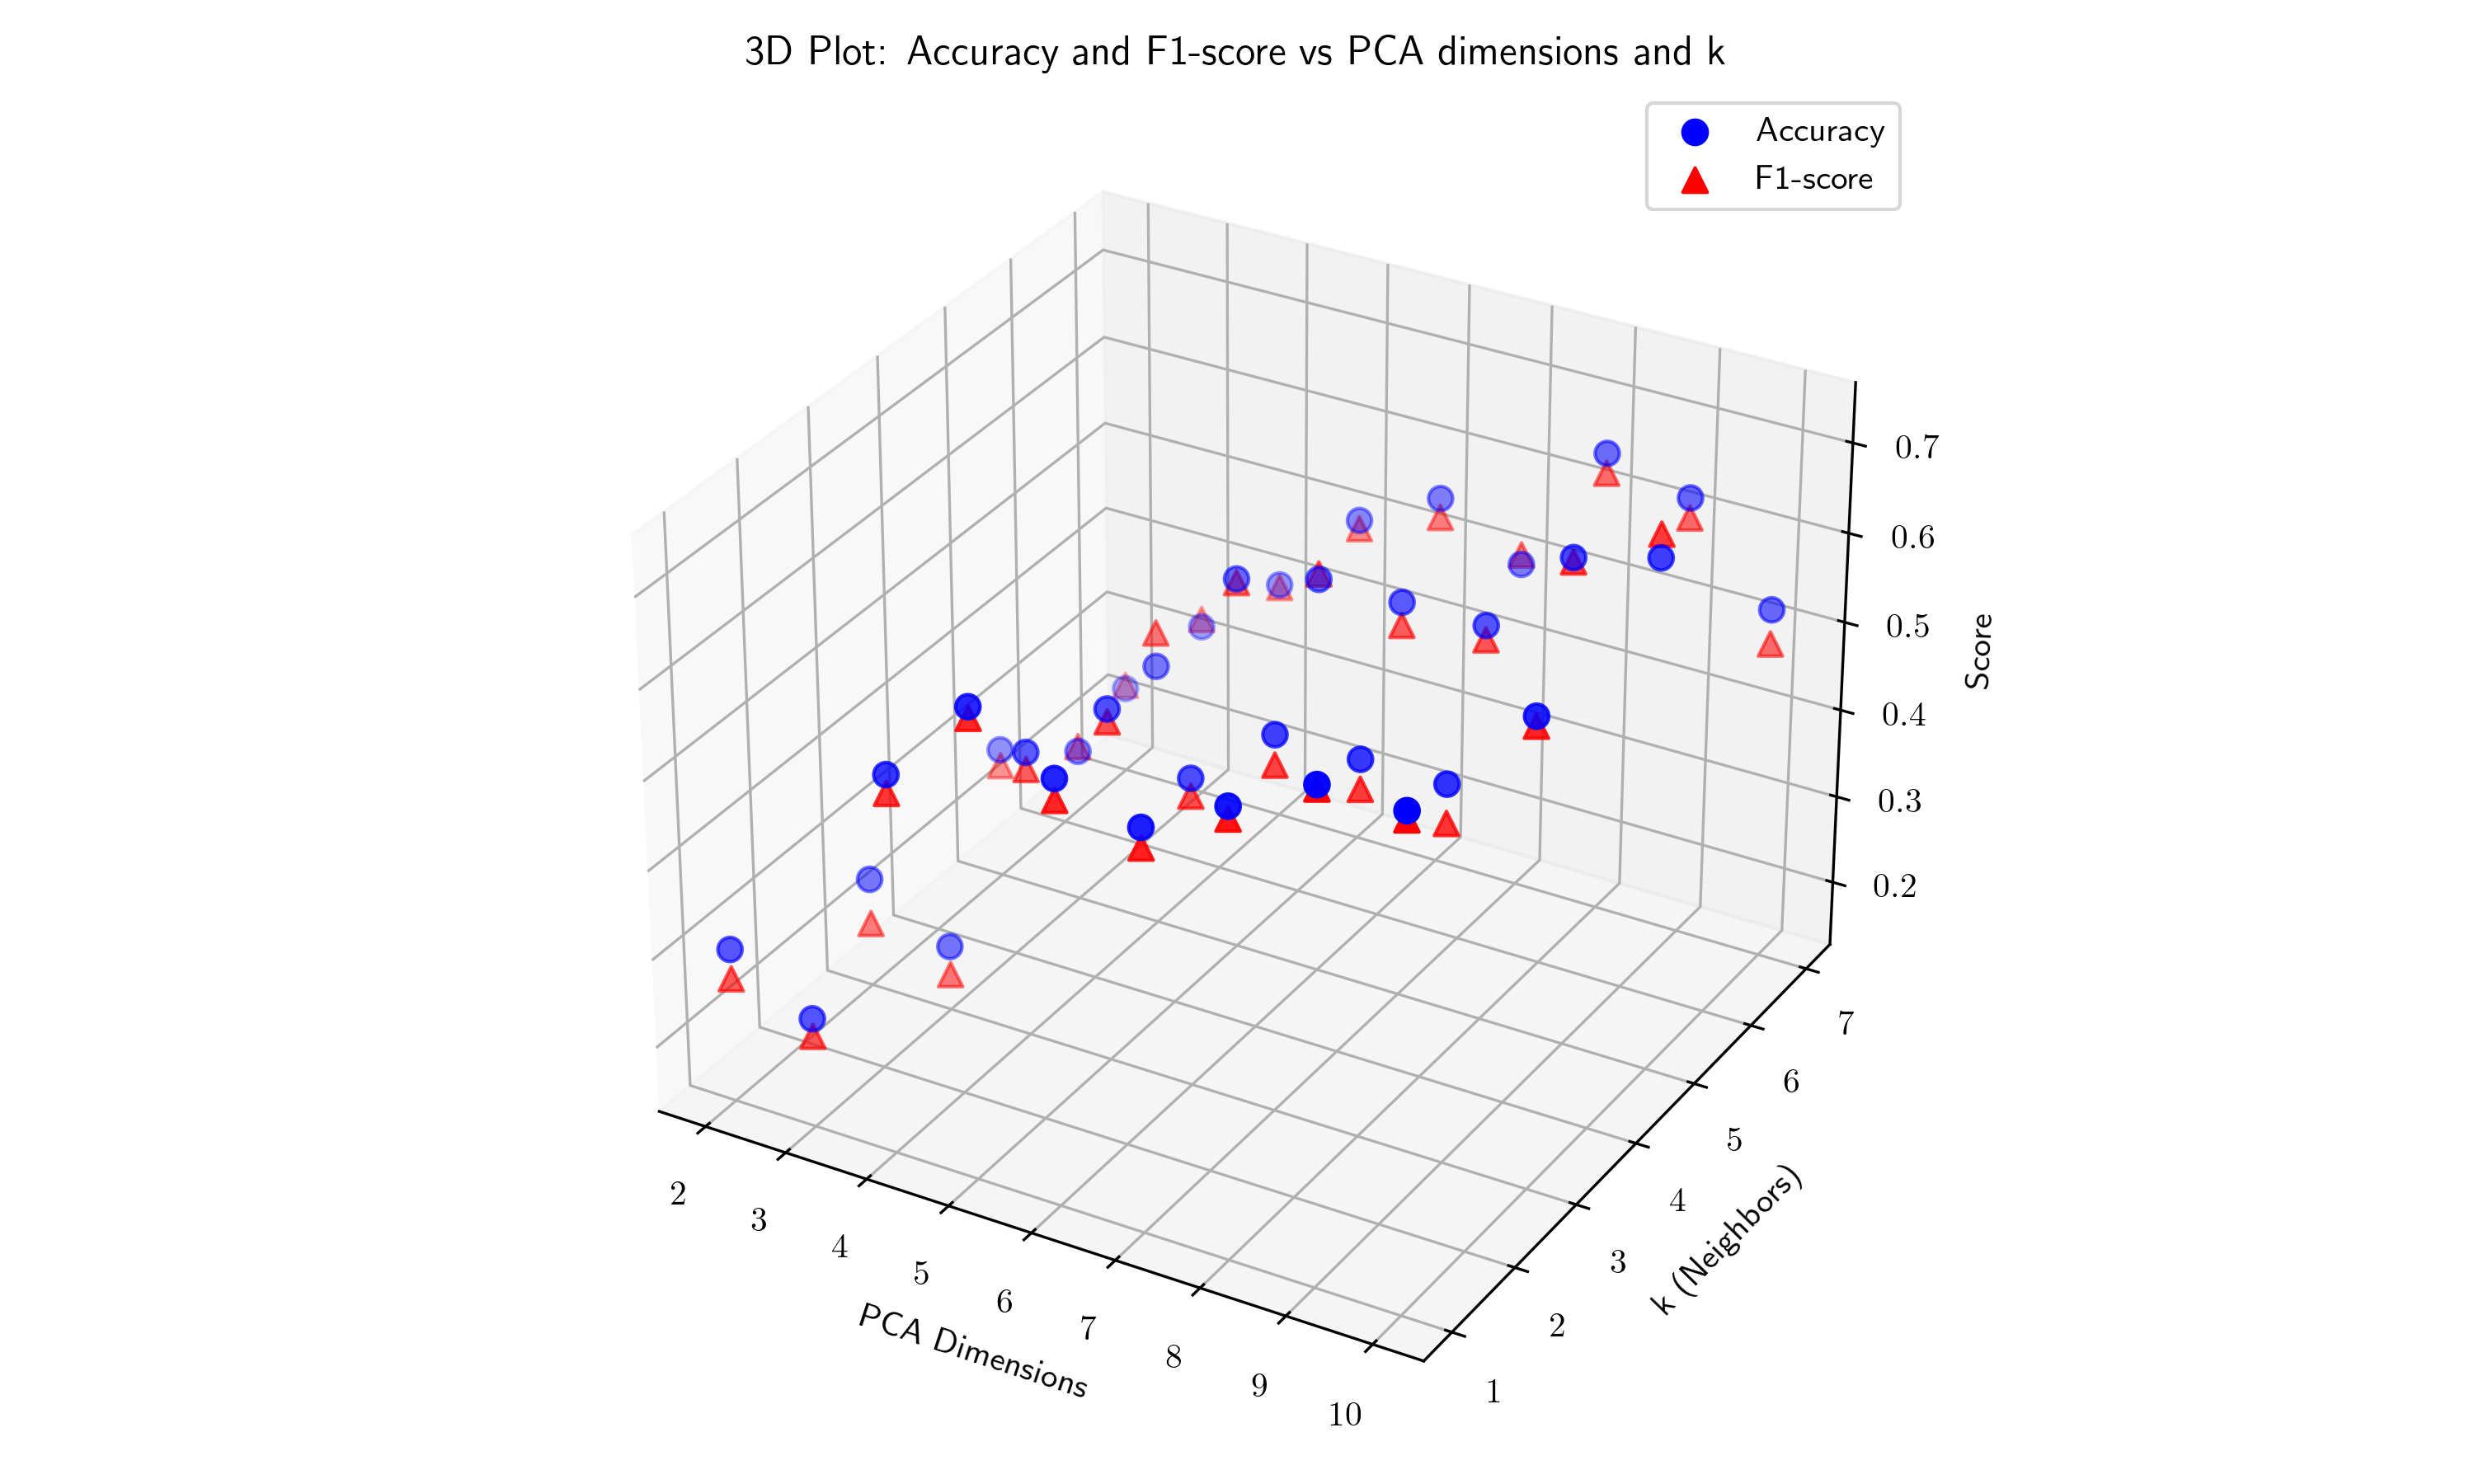
\includegraphics[width=\linewidth]{plots/3D_accuracy_f1_knn_step7.png}
\end{figure}

\noindent Το τελευταίο μοντέλο που δοκιμάζουμε είναι το Logistic Regression (\lstinline[language=Python]{LogisticRegression()}). Παραθέτουμε πάλι το αντίστοιχο διάγραμμα. Το καλύτερο μοντέλο λήφθηκε για 6 συνιστώσες με ακρίβεια 65\%.

\begin{figure}[H]
	\centering
	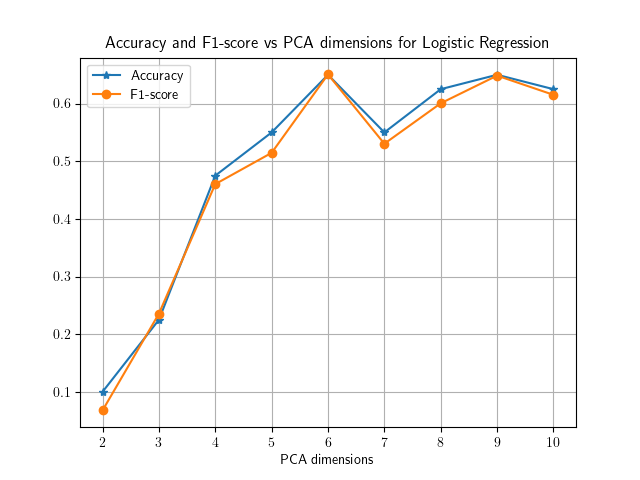
\includegraphics[width=\linewidth]{plots/accuracies_and_f1_lr_step7.png}
\end{figure}

\subsection*{Bonus}

Αυτό που θα κάνουμε είναι να προσθέσουμε επιπλέον πληροφορία στο διάνυσμα χαρακτηριστικών (εκτός από mean mfcc, delta και delta\_deltas) όπως το zero-crossing rate. Για αυτό τροποποιούμε την συνάρτηση εξαγωγής των mfcc και των παραγώγων τους έτσι ώστε εκτός από αυτά να μας επιστρέφει και τα zero crossings και spectral centroids. Τέλος υλοποιούμε και μία συνάρτηση για την σύγκριση της επίδοσης των ταξινομητών που χρησιμοποιήσαμε παραπάνω σε αυτά τα νέα επαυξημένα δείγματα. Τα βήματα που ακολουθούμε scaling και PCA είναι ίδια με πριν. Γενικά, αυτό που ελπίζουμε εισάγοντας επιπλέον χαρακτηριστικά είναι να κάνουμε τα δείγματά μας περισσότερο διαχωρίσιμα. Αυτό πράγματι θα γίνει εφόσον τα χαρακτηριστικά αυτά που θα επιλέξουμε είναι ασυσχέτιστα μεταξύ τους (δεν κουβαλούν redundant πληροφορία), αλλά και ασυσχέτιστα με εκείνα που έχουμε ήδη επιλέξει. Προφανώς, όποια χαρακτηριστικά και να επιλέξουμε να προσθέσουμε δεν θα πετύχουμε και τα 2 στον μέγιστο βαθμό. Έτσι, αναμένουμε οι μετρικές μας να βελτιωθούν αλλά όχι δραματικά. Στις δοκιμές που κάναμε το καλύτερο αποτέλεσμα πάρθηκε από τον ταξινομητή Logistic Regression - Accuracy 80\%. Επιπλέον, η προσδοκία μας, κατά κανόνα, επιβεβαιώνεται αφού η ακρίβεια βελτιώνεται, αλλά όχι πάνω από 7.5\%. Στη επόμενη σελίδα παρουσιάζουμε μία σύγκριση της απόδοσης των ταξινομητών πριν και μετά την εισαγωγή των επιπλέον features αλλά και το πόσες διαστάσεις είναι καλύτερο να διατηρήσουμε μετά το PCA. \\

\noindent Αξίζει να επισημάνουμε ότι το Logistic Regression παρουσιάζει και χωρίς τα επιπλέον features καλύτερη επίδοση και από το μη bonus ερώτημα. Αυτό γίνεται διότι ο αριθμός των διαστάσεων χαρακτηριστικών που του δίνονται είναι 40 και 35 αντίστοιχα, πολύ μεγαλύτερος από το προηγούμενο μέγιστο, δηλαδή 10.

\begin{figure}[H]
	\centering
	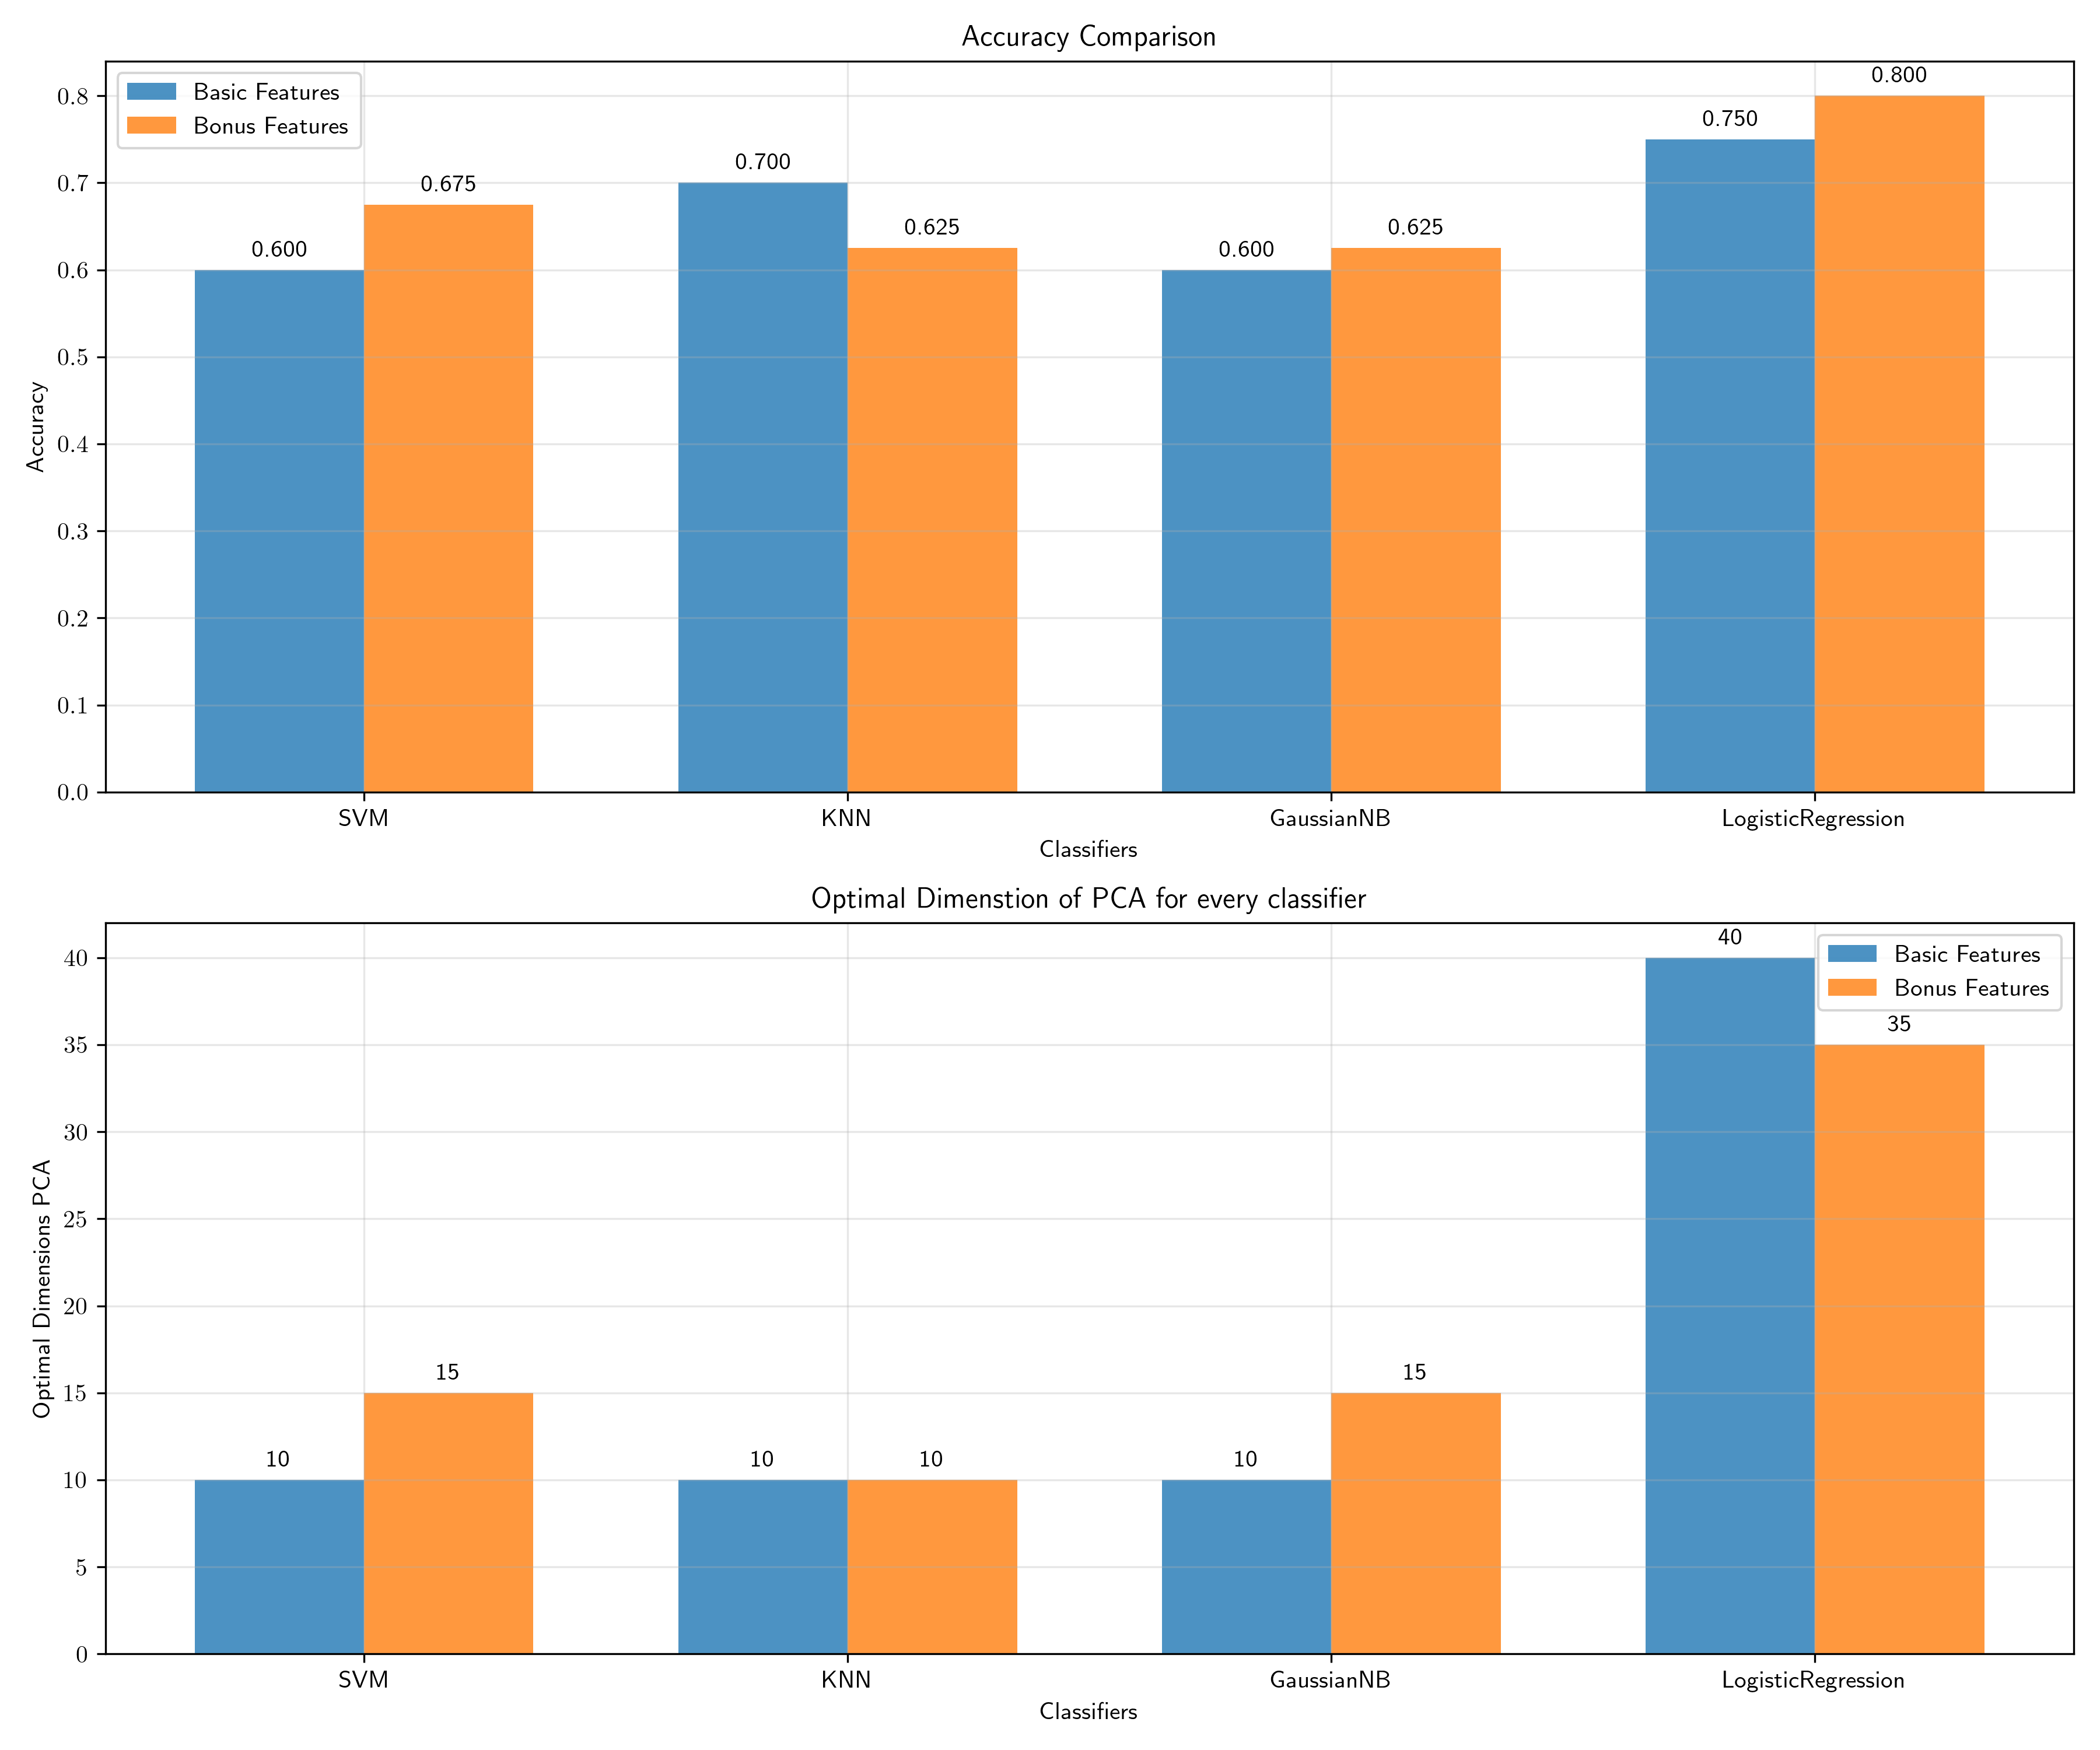
\includegraphics[width=\linewidth]{plots/bonus_features_comparison_with_pca.png}
\end{figure}





\section*{Βήμα 8}
Σε αυτό το βήμα μας ζητείται να δημιουργήσουμε ακολουθίες 10 σημείων ενός ημιτόνου και ενός συνημιτόνου συχνότητας 40Hz. Στόχος είναι να προβλέψουμε τις ακολουθίες συνημιτόνου έχοντας ως δεδομένες εκείνες των ημιτόνων. \\

\noindent Για να το πετύχουμε αυτό επιστρατεύουμε 3 είδη νευρωνικών δικτύων, το RNN, το LSTM και το GRU. Για να τα ορίσουμε και να τα εκπαιδεύσουμε αξιοποιούμε την PyTorch.

\begin{itemize}
	\item \textbf{RNN:} Πρόκειται για ένα τύπο νευρωνικού δικτύου ειδικά σχεδιασμένου ώστε να επεξεργαστούμε ακολουθιακά δεδομένα και να ανιχνεύσουμε τις εξαρτήσεις τους και τα μοτίβα τους στο χρόνο.
	
	\begin{figure}[h]
		\centering
		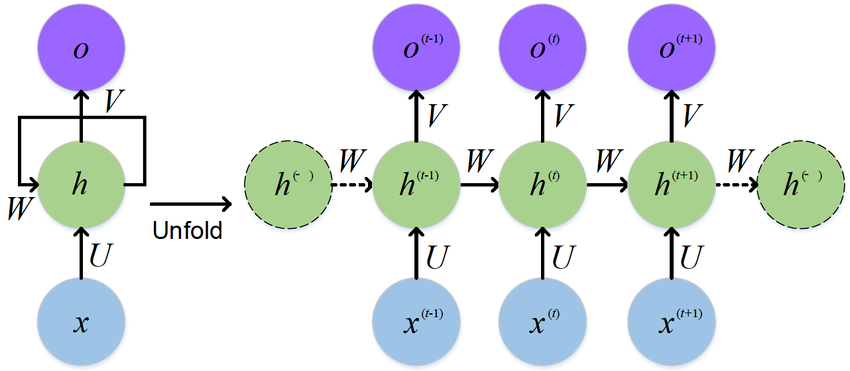
\includegraphics[width=0.5\linewidth]{plots/rnn.png}
	\end{figure}
	
	Ο κώδικας του ορισμού του είναι ο εξής: \\
	\lstinputlisting[language=Python]{scripts/rnn.py} 
	
	Ουσιαστικά έχουμε το component που υλοποιοεί ένα RNN, το οποίο πρσφέρεται έτοιμο από την PyTorch και κατόπιν ένα fully connected layer το οποίο συνδυάζει τα outputs των hidden layers του RNN κάθε χρονική στιγμή-δείγμα και μας δίνει το τελικό προβλεπόμενο output για τη δεδομένη χρονική στιγμή. 
	
	\item \textbf{LSTM:} Το LSTM είναι ένα είδος RNN το οποίο αναπτύχθηκε προκειμένου να αντιμετωπίσει το πρόβλημα του vanishing gradient που εμφανιζόταν έντονα στον πρόγονό του. Ουσιαστικά, δίνει δυνατότητα short term memory στο μοντέλο ώστε να "θυμάται" πληροφορίες και εξαρτήσεις στα δεδομένα για χιλιάδες δείγματα, σε αντίθεση με το RNN το οποίο "έχανε" τις εξαρτήσεις δεδομένων που απείχαν κάποιο μεγάλο αριθμό δειγμάτων (αυτό είναι το manifestation του vanishing gradient).
	
	\begin{figure}[h]
		\centering
		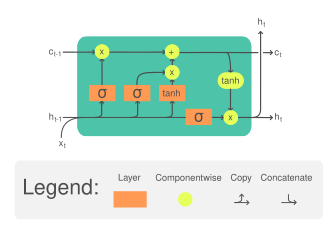
\includegraphics[width=0.5\linewidth]{plots/lstm.png}
	\end{figure}
	
	Ο κώδικας του ορισμού του φαίνεται παρακάτω και ακολουθεί τη λογική του RNN: \\
	\lstinputlisting[language=Python]{scripts/lstm.py}
	
	\item \textbf{GRU:} Είναι και αυτό "απόγονος" του RNN. Πρακτικά μοιάζει με το LSTM, μόνο που έχει έναν μηχανισμό από πύλες στο input, αλλά δεν έχει πύλη στο output και συνεπώς έχει λιγότερες παραμέτρους από το LSTM. 
	
	\begin{figure}[h]
		\centering
		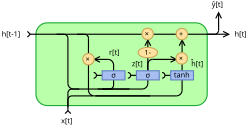
\includegraphics[width=0.5\linewidth]{plots/gru.png}
	\end{figure}
	
	Ο κώδικας του ορισμού του φαίνεται παρακάτω και ακολουθεί τη λογική του RNN και του LSTM: \\
	\lstinputlisting[language=Python]{scripts/gru.py}
\end{itemize}

\noindent Στην συνέχεια, εκπαιδεύουμε τα μοντέλα μας και συγκρίνουμε την απόδοσή τους. Η διαδικασία που ακολουθούμε είναι η εξής:

\begin{enumerate}
	\item \textbf{Δημιουργία δειγμάτων ημιτόνων και συνημιτόνων:} \\
	Με την NumPy δημιουργόυμε τα σήματα-εισόδους για τα νευρωνικά δίκτυα μας καθώς και τα σήματα-στόχους που θέλουμε να προβέψουμε (t = np.linspace(0, 1, total\_points),
	x = np.sin(2*np.pi*f*t), y = np.cos(2*np.pi*f*t))
	
	\item \textbf{Εκπαίδευση των μοντέλων:} \\
	\lstinputlisting[language=Python]{scripts/trainning.py}
	
	Ως κριτήριο ελαχιστοποίησης επιλέξαμε το Mean Square Error ενώ για optimizer τον Adam. O Adam ενσωματώνει και όρους ορμής στην δική του υλοποίηση του gradient descend. Εκπαιδεύουμε όλα τα μοντέλα για 100 εποχές. \\
	Αρχικά, πριν από κάθε εποχή πρέπει να καθαρίσουμε τα προηγούμενα gradients γιατί η default συμπεριφορά της PyTorch είναι να τα συσσωρεύει, όχι να τα πανωγράφει. \\
	Στη συνέχεια, υπολογίζουμε το output του μοντέλου και το loss (αντίστοιχο της απόκλισης από το στόχο μας). Τέλος κάνουμε backpropagation τα loss gradients και ενημερώνουμε τα βάρη. \\
	Τα losses αποθηκεύονται ώστε να χρησιμοποιηθούν σε διαγράμματα μετέπειτα.
	
	\item \textbf{Αξιολόγηση των μοντέλων:} \\
	\lstinputlisting[language=Python]{scripts/eval.py}
	Αρχικά, βάζουμε το μοντέλο σε eval mode (από documentation της PyTorch) και κατόπιν απενεργοποιούμε τον υπολογισμό και την αποθήκευση των gradients διότι αυτή η υπολογιστικά ακριβή διαδικασία δεν είναι απαραίτητη κατά το inference. Τέλος υπολογίζουμε τις μετρικές μας για τα test samples και τις επιστρέφουμε.
\end{enumerate}

\subsection*{Αποτελέσματα}

\begin{figure}[h]
	\centering
	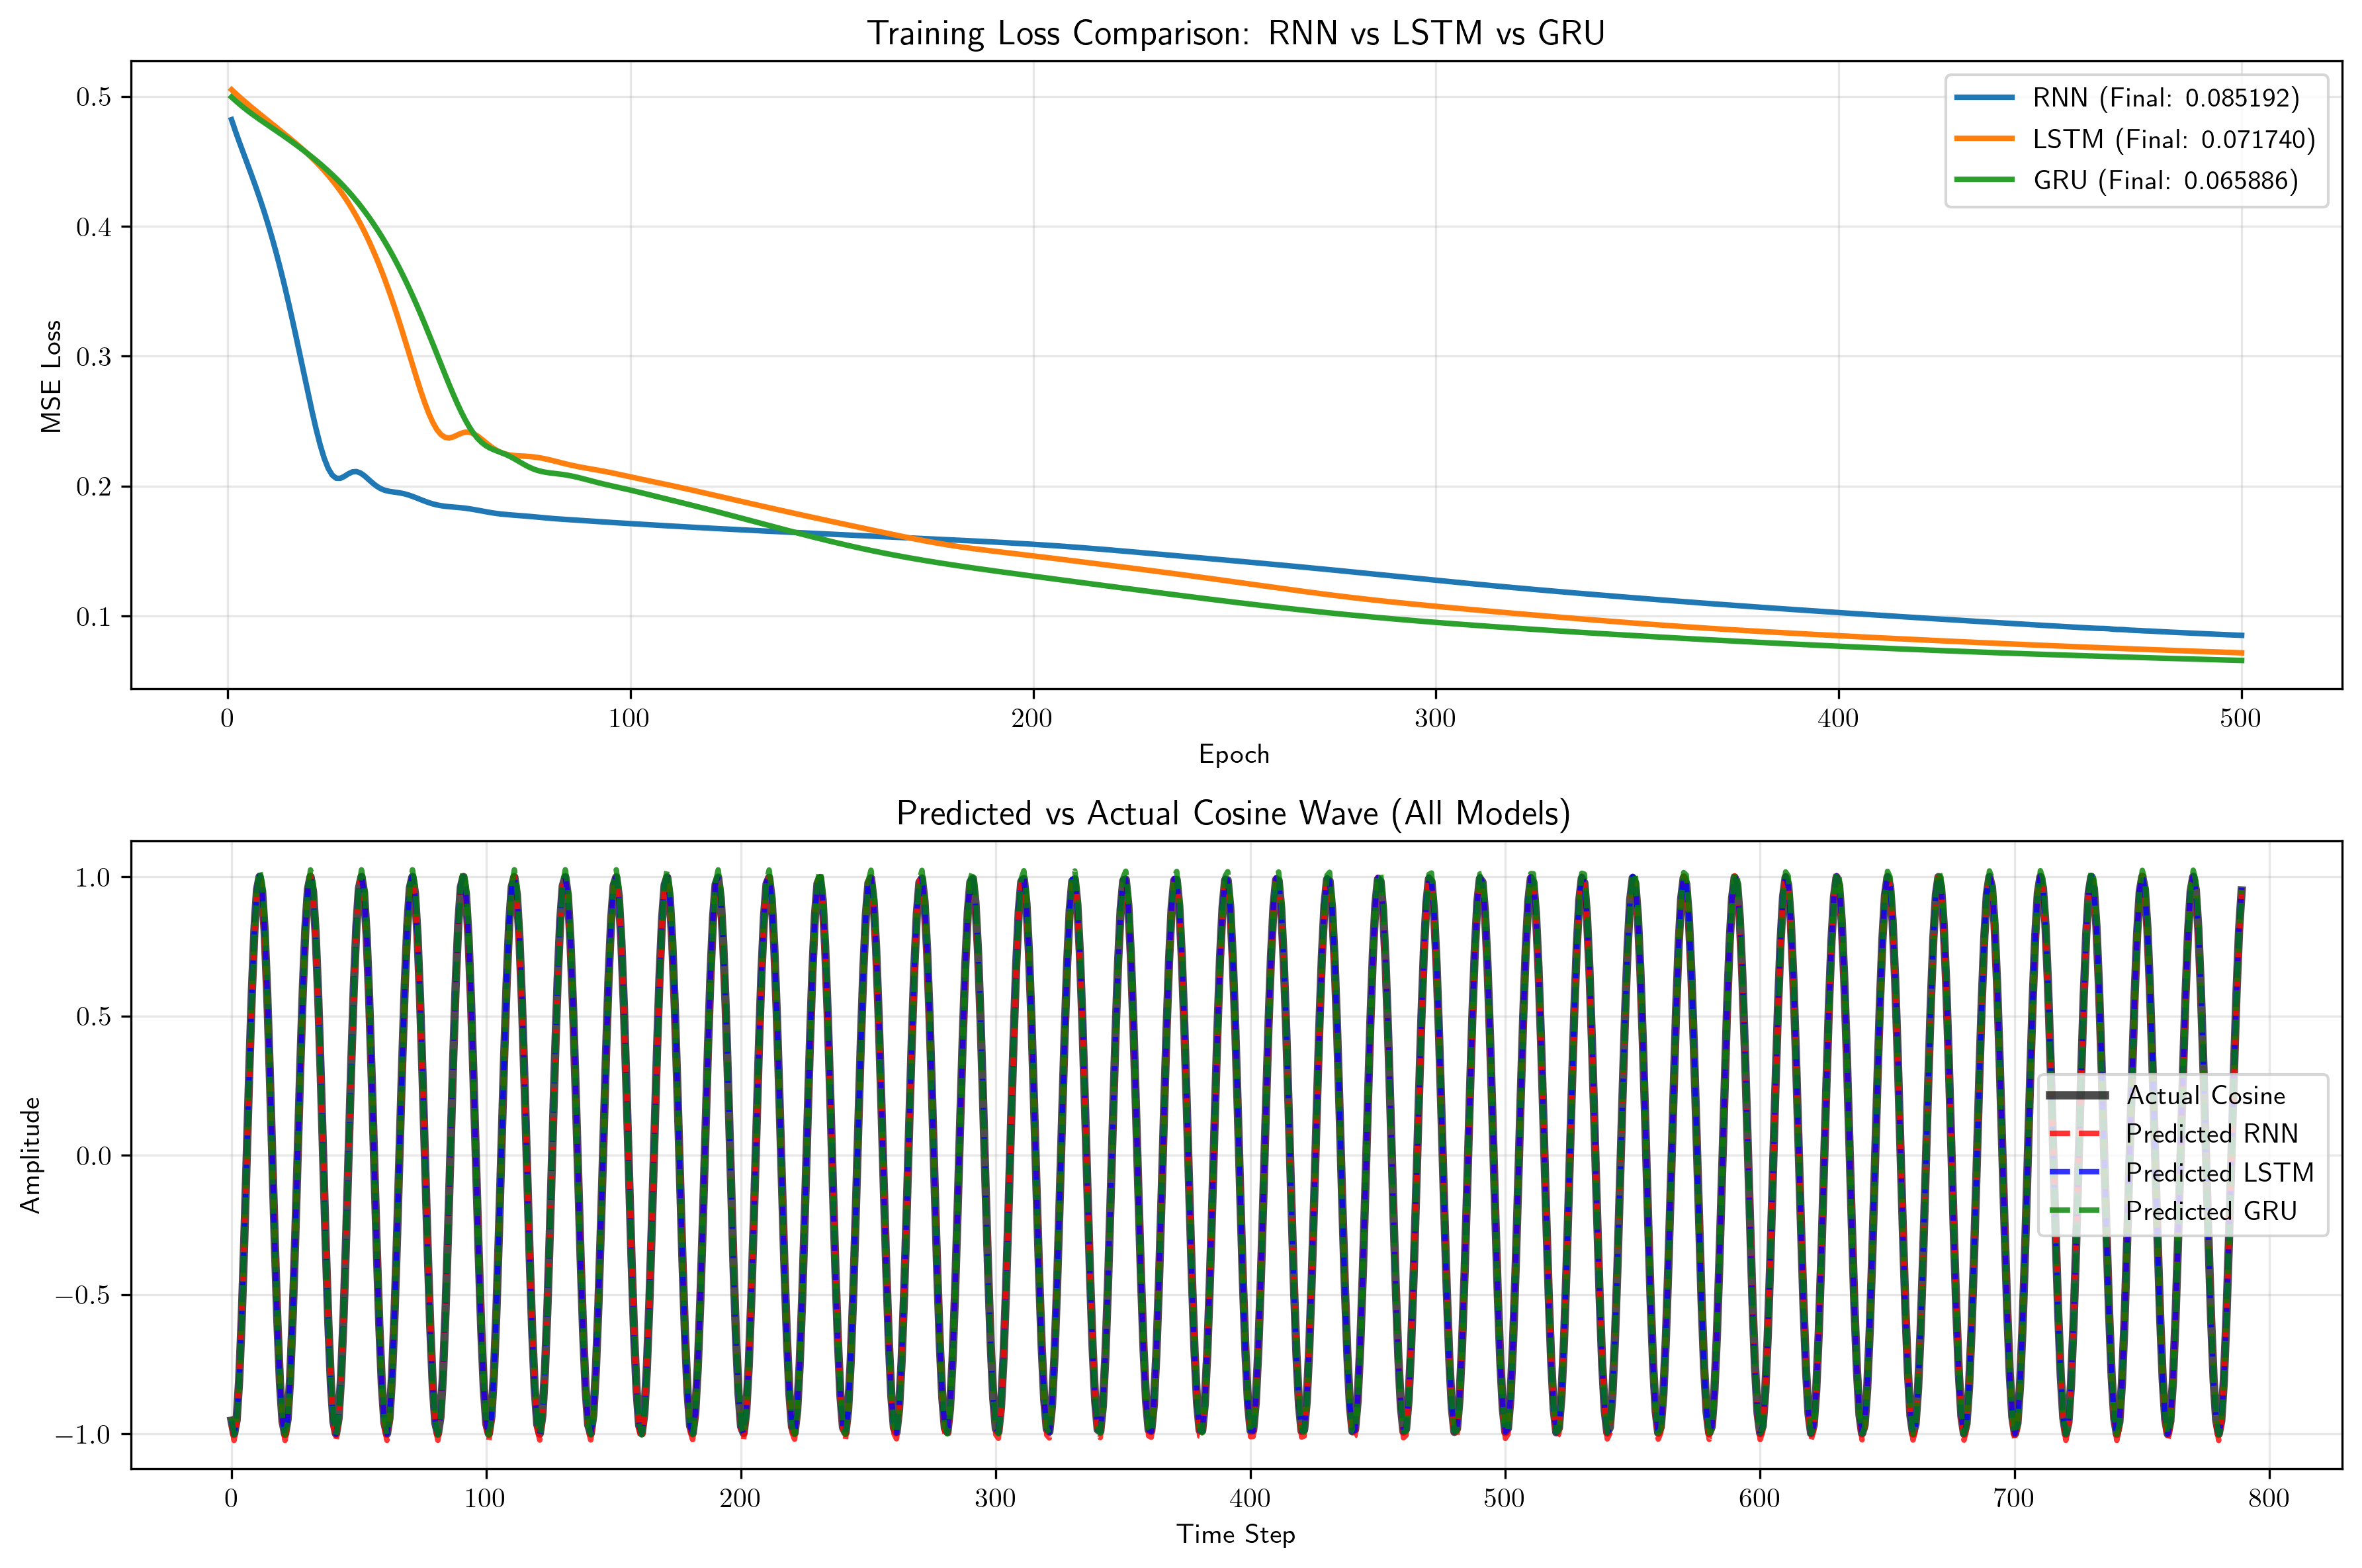
\includegraphics[width=0.9\linewidth]{plots/final_all_models_comparison.png}
\end{figure}

\noindent Σε αυτό το γράφημα εξετάζουμε τη συμπεριφορά των μοντέλων κατά την εκπαίδευσή τους και παίρνουμε μια πρώτη εικόνα για το κατά πόσο το αποτέλεσμα είναι ικανοποιητικό. \\

\noindent Βλέπουμε ότι έχουμε εκπαιδεύσει τα μοντέλα μας για 500 εποχές. Καταλήξαμε σε αυτή την επιλογή ως εξής:

\begin{enumerate}
	\item Αρχικά, εκπαιδεύσαμε με 100 εποχές. Αυτό οδήγησε στο εξής παράδοξο: Το RNN, θεωρητικά το πιο "αδύναμο" μοντέλο είχε το μικρότερο loss - δηλαδή είχε προσαρμοστεί καλύτερα στα δεδομένα. Αυτό μπορεί να έχει μόνο μία εξήγηση, δεδομένου ότι έχει μικρότερη χωρητικότητα από τα προηγούμενα 2. Ο μεγαλύτερος αριθμός παραμέτρων των LSTM και GRU δεν τους έχει επιτρέψει να συγκλίνουν ακόμα. Οπότε αυξάνουμε τον αριθμό εποχών σε 300.
	
	\item Όπως φαίνεται και στο plot παραπάνω, μετά τις 180 εποχές πράγματι τόσο το LSTM όσο και το GRU έχουν μικρότερο loss από το RNN. Αλλά βλέπουμε ότι το loss έχει την τάση να μειωθεί κι άλλο. Οπότε αυξάνουμε σε 500 εποχές
	
	\item Βλέπουμε ότι το loss δεν βελτιώνεται οπότε σταματάμε (σε αυτό το σημείο θα μπορούσαμε να αρχίσουμε να αυξάνουμε τα hidden layers).
\end{enumerate}

\noindent Αφότου εξηγήσαμε την διαδικασία της εκπαίδευσής μας, βλέπουμε ότι και το αποτέλεσμα για τα μοντέλα μας, οπτικά, είναι αρκετά υποσχόμενο. Για να το επιβεβαιώσουμε πλήρως εξετάζουμε το αποτέλεσμα σε ένα zoom της κυματομορφής για κάθε μοντέλο ξεχωριστά.

\begin{figure}[H]
	\centering
	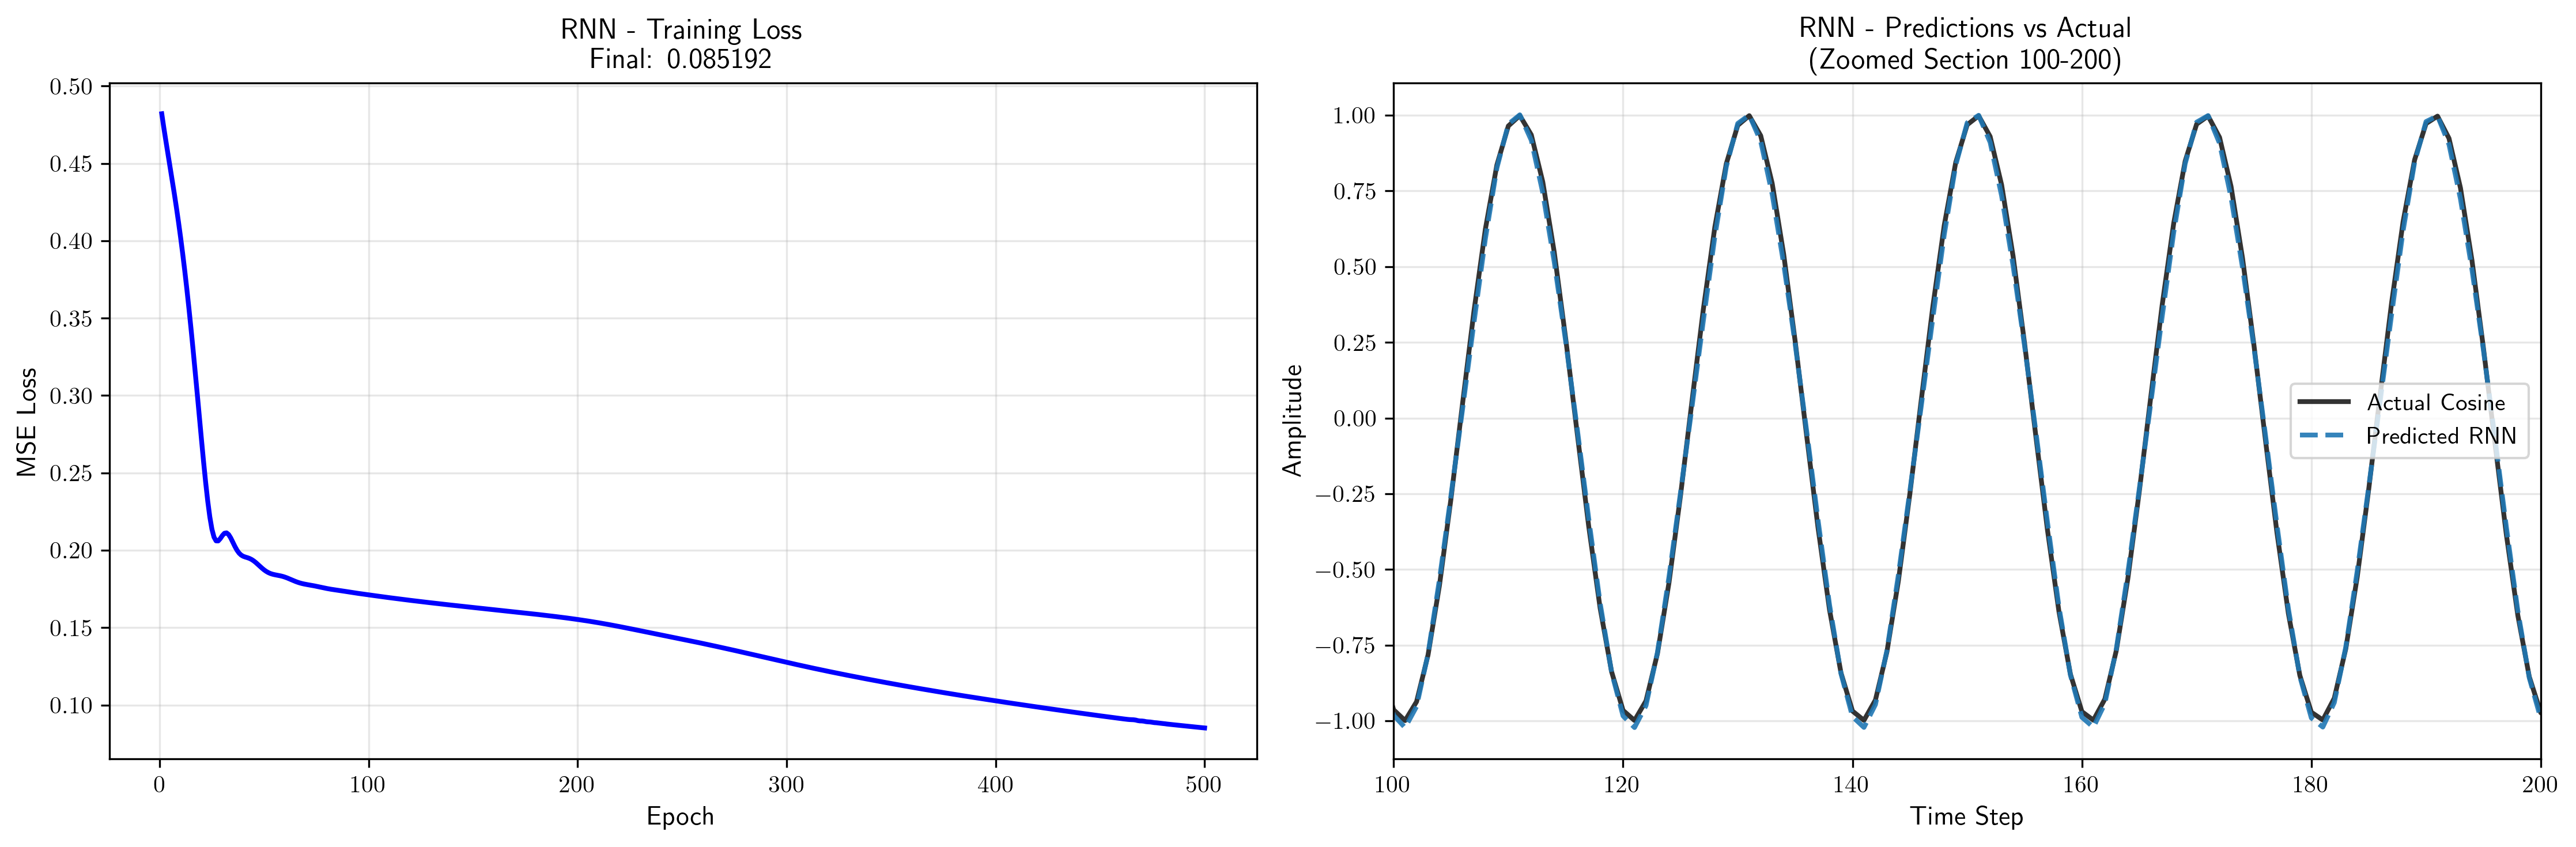
\includegraphics[width=0.9\linewidth]{plots/rnn_clean.png}
\end{figure}

\begin{figure}[H]
	\centering
	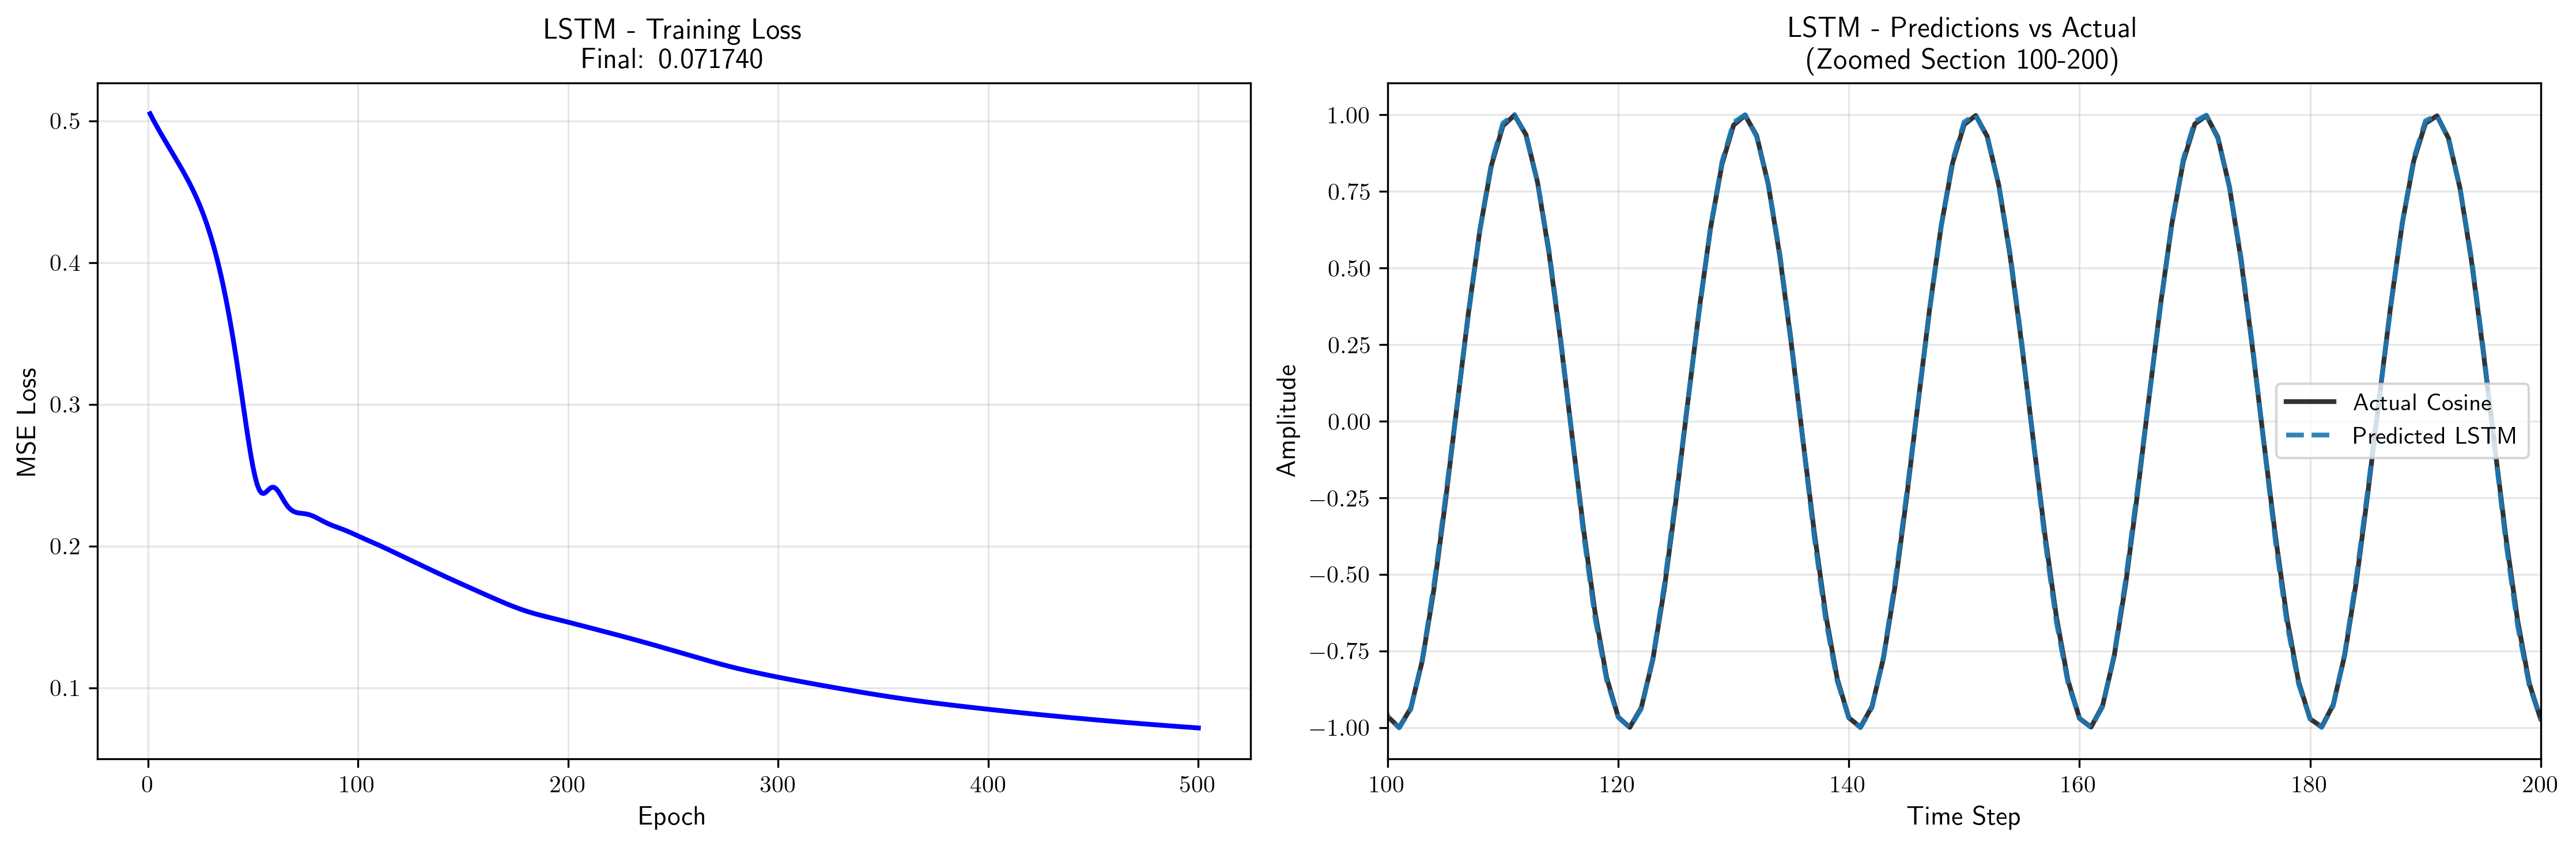
\includegraphics[width=0.9\linewidth]{plots/lstm_clean.png}
\end{figure}

\begin{figure}[H]
	\centering
	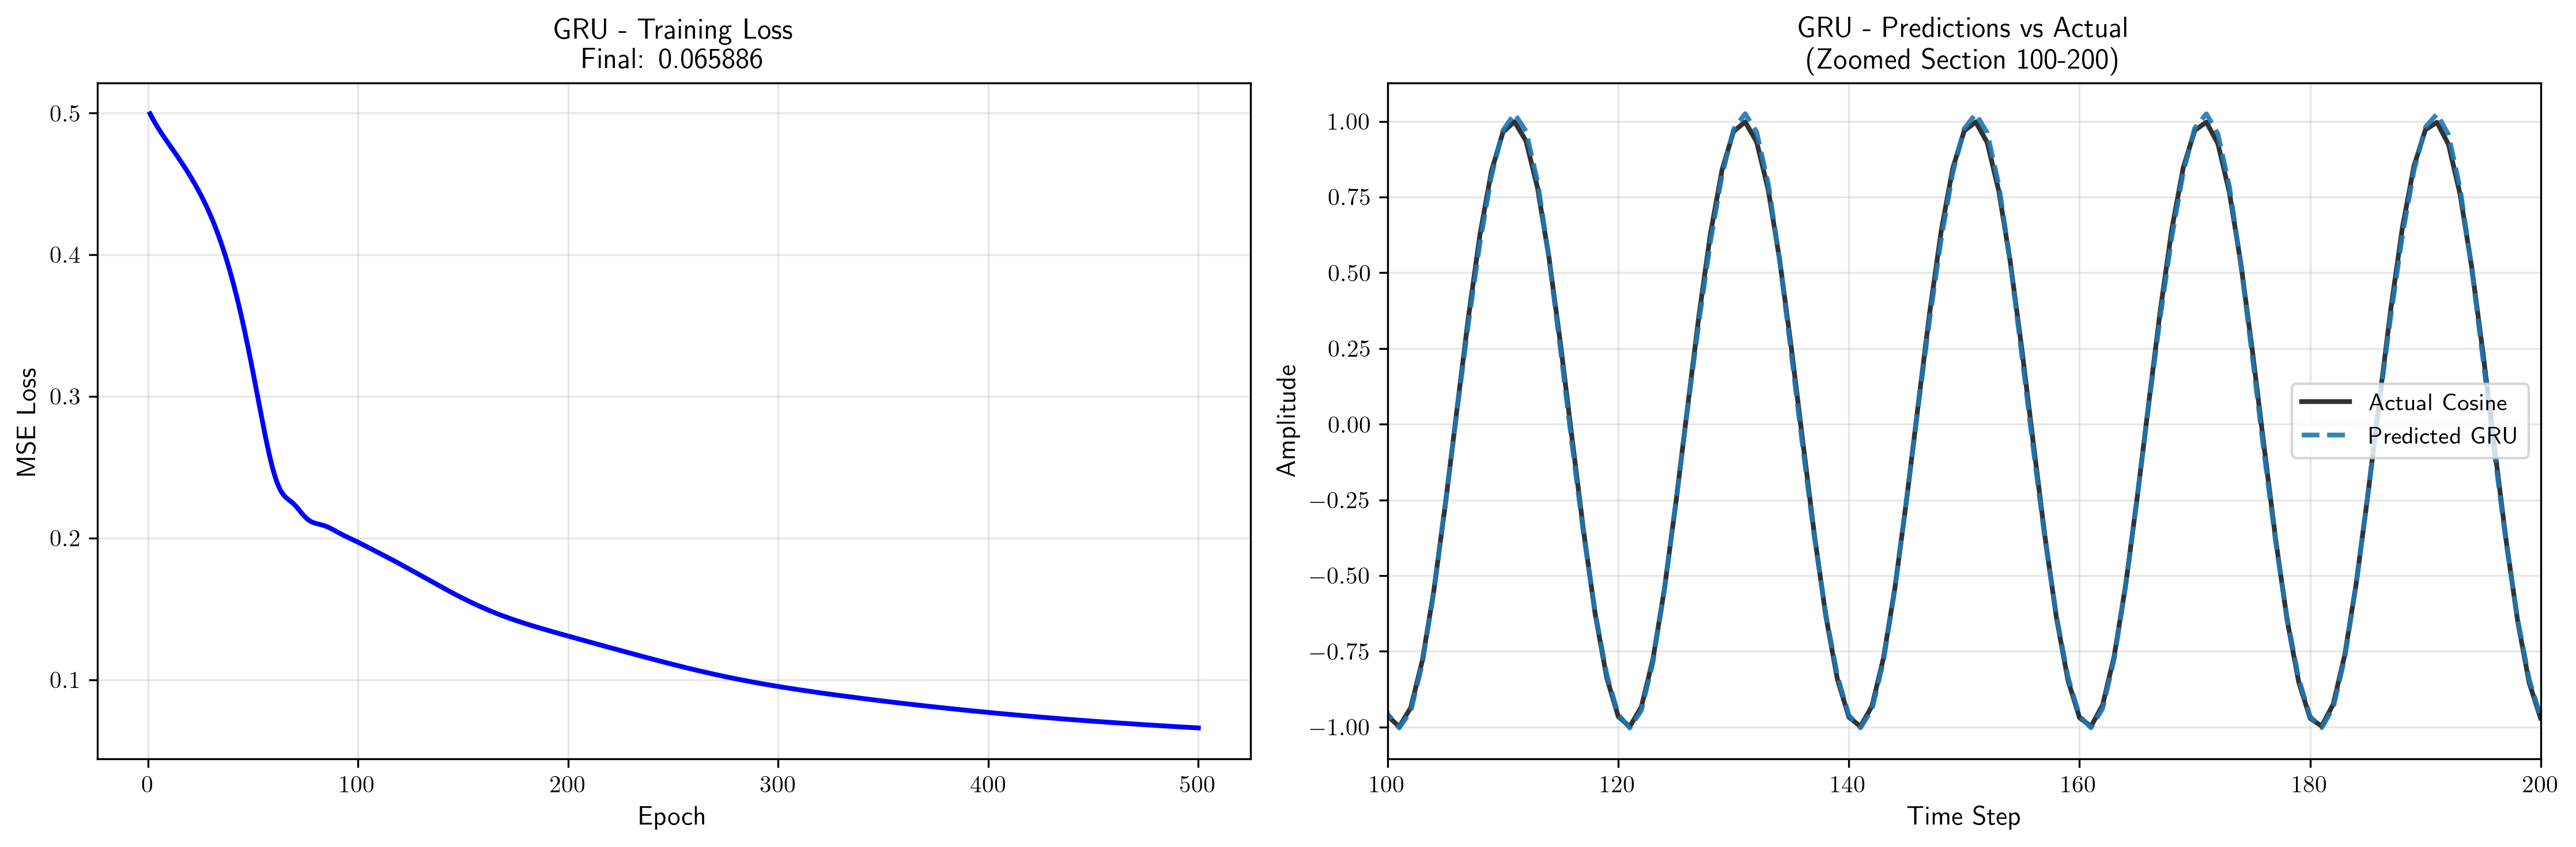
\includegraphics[width=0.9\linewidth]{plots/gru_clean.png}
\end{figure}

\noindent Και για τα 3 μοντέλα το αποτέλεσμα είναι πολύ ικανοποιητικό. \\

\noindent Τέλος, επιλέγουμε το καλύτερο μοντέλο με βάση το μικρότερο MSE στο test set. Αυτό βλέπουμε ότι είναι το GRU.

\begin{figure}[H]
	\centering
	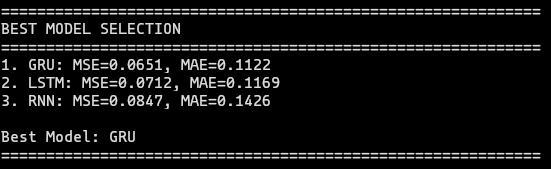
\includegraphics[width=0.5\linewidth]{plots/best_model_selection.png}
\end{figure}

\section*{Βήμα 9}

Πρώτα από όλα κάνουμε clone τα δεδομένα σε μορφή .wav από το repository της εργασίας στον υπολογιστή μας. \\

\noindent Στη συνέχεια, αξιοποιύμε τον βοηθητικό κώδικα του εργαστηρίου προκειμένου να υλοποιήσουμε τα επόμενα βήματά μας (\textit{parser.py, hmm.py})

\lstinputlisting[language=Python, firstline=138, lastline=162]{../../lab.py}

\noindent Όπως φαίνεται και στη συνάρτηση παραπάνω, διαβάζουμε από το φάκελο τα wav αρχεία και εξάγουμε 13 MFCC για το καθένα. Στη συνέχεια με την έτοιμη συνάρτηση split του κώδικα τη χωρίζουμε στο default train test split το οποίο έχει 2700 από τα 3000 δείγματα ακολουθιών στο train και τα υπόλοιπα στο test. Στη συνέχεια, καλούμαστε να χωρίσουμε το test set αυτό σε 2 μικρότερα. Ένα validation και ένα test set σε αναλογία 80-20 αντίστοιχα. Αυτό, όπως φαίνεται και στον κώδικα παραπάνω, γίνεται με τη χρήση του \textit{train\_test\_split}. Η παράμετρος stratify μας εξασφαλίζει την ομοιόμορφη κατανομή των δειγμάτων. Δηλαδή, ότι θα έχουμε τον ίδιο αριθμό ψηφίων από κάθε κατηγορία. Έτσι αποφεύγουμε biases.

\begin{figure}[H]
	\centering
	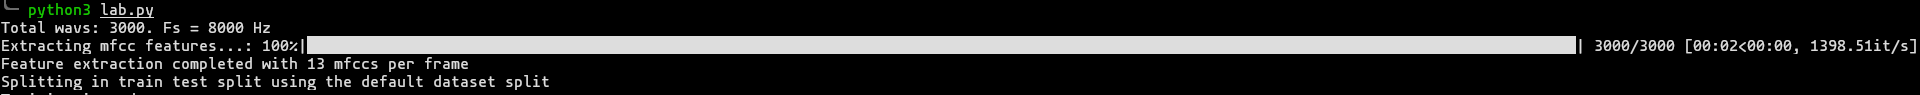
\includegraphics[width=\linewidth]{images/step9.png}
	\caption{Ανάγνωση Dataset}
\end{figure}




\section*{Βήμα 10}

Στο βήμα αυτό υλοποιούμε αναγνώριση ψηφίων από ομιλία με GMM-HMM. Η λειτουργία του μοντέλου φαίνεται διαγραμματικά παρακάτω:

\begin{figure}[H]
	\centering
	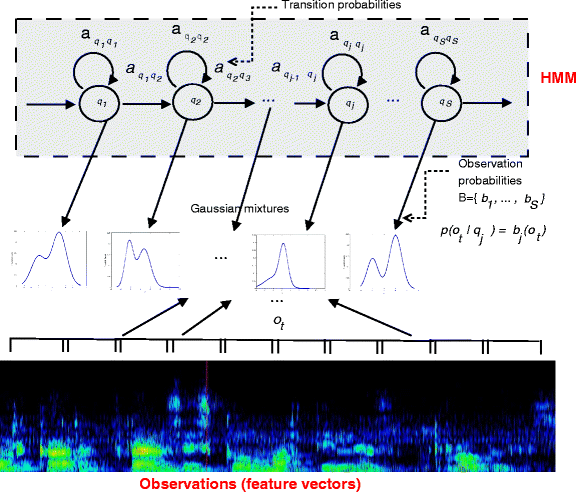
\includegraphics[width=0.75\linewidth]{images/GMM_HMM_diagram.png}
	\caption{Image by \cite{HMM_GMM_image}}
\end{figure}

\noindent Δημιουργούμε ένα HMM ανά ψηφίο, οπότε η έξοδος του i-οστού HMM θα είναι η πιθανότητα το σήμα να αντιστοιχεί στο i-οστό ψηφίο. Οι παρατηρήσεις σε κάθε state του HMM είναι ένα διαφορετικό mixture of gaussians. Αφού εκπαιδευτεί το GMM από μόνο του σε όλα τα δεδομένα, θα εκπαιδευτεί από κοινού το GMM-HMM μοντέλο και το μείγμα κατανομών ανά state θα γίνει fit στην παρατήρηση που συμβαίνει σε αυτό το state. Ιδανικά, θα θέλαμε εξ'αρχής να μην εκπαιδεύουμε το GMM σε όλα τα δεδομένα, αλλά μόνο σε αυτά που αντιστοιχούν στο χρονικό διάστημα που περιγράφεται από το state. Κάτι τέτοιο, όμως, είναι δυστυχώς δύσκολο να γίνει, αφού δεν είναι προκαθορισμένο για κάθε ψηφίο το πότε θα γίνει η μετάβαση από το ένα state στο επόμενο, οπότε θα αρκεστούμε στην διαφοροποίηση μεταξύ των GMMs που κάνει στη συνέχεια η από κοινού εκπαίδευση. Τέλος, σημειώνουμε ότι με το μείγμα γκαουσιανών μοντελοποιούμε την κατανομή των MFCCs ανά ψηφίο και state, αφού περιμένουμε πως η κάθε τέτοια κατανομή δεν θα είναι unimodal στον χώρο των MFCCs λόγω των διαφορών στην εκφώνηση του ίδιου ψηφίου μεταξύ διαφορετικών ομιλητών.\\
\\
\noindent Η συνάρτηση train φαίνεται παρακάτω:

\lstinputlisting[language=Python, firstline=260, lastline=270]{../../lab.py}

\noindent Την \verb*|initialize_and_fit_normal_distributions| καθώς είναι υποπερίπτωση του GMM για n\_mixtures = 1.\\
\\
\noindent Η αρχική εκπαίδευση του GMM γίνεται ως εξής:

\lstinputlisting[language=Python, firstline=165, lastline=197]{../../lab.py}

\noindent Δηλαδή αρχικοποιούμε κάθε γκαουσιανή σε multivariate gaussian με μέσο ειλημμένο από D-διάστατη τυπική κανονική κατανομή, όπου D η διάσταση των δεδομένων, εδώ 13 για τα MFCCs, και με συνδιασπορά τον D-διάστατο ταυτοτικό πίνακα. Επίσης περιορίζουμε κατά την εκπαίδευση τον πίνακα συνδιασποράς να είναι διαγώνιος, ώστε να μειώσουμε τις παραμέτρους και τον χρόνο εκπαίδευσης αλλά και να έχουμε πιο απλές αναπαραστάσεις για τα δεδομένα μας.\\
\\
\noindent Αντίστοιχα, το HMM το εκπαιδεύουμε ως εξής:

\lstinputlisting[language=Python, firstline=241, lastline=257]{../../lab.py}

\noindent Για πίνακα μετάβασης χρησιμοποιήσαμε τον $A = [α_{i, j}]_{1 \le i, j \le n}$, όπου $n = \text{n\_states}$ το πλήθος καταστάσεων στα HMMs, με:
$$α_{i, j} = 
\begin{cases}
	1, & \text{if $j = i = n$}\\
	0.8 & \text{if $j = i \neq n$}\\
	0.2 & \text{if $j = i+1$}\\
	0 & \text{αλλιώς}
\end{cases}
$$

\noindent Οι τιμές 0.8 για την ανακύκλωση και 0.2 για την μετάβαση επιλέχθηκαν επειδή το μοντέλο πιο συχνά θα επιλέγει να μείνει στην ίδια κατάσταση, παρά να μεταβεί στην επόμενη.

\lstinputlisting[language=Python, firstline=212, lastline=222]{../../lab.py}

\noindent Τέλος, αρχικοποιήσαμε τις πιθανότητες εκκίνησης ως $1$ στην αρχική κατάσταση και $0$ σε όλες τις άλλες, ενώ τις πιθανότητες τερματισμού ως $1$ στην τελική κατάσταση και $0$ σε όλες τις άλλες.

\lstinputlisting[language=Python, firstline=225, lastline=238]{../../lab.py}

\section*{Βήμα 11}

Πλέον, έχουμε υλοποιήσει τα μοντέλα, οπότε μπορούμε να τα εκπαιδεύσουμε στο training set και να ελέγξουμε την απόδοση του καθενός στο validation set. Η εκπαίδευση κάθε GMM-HMM γίνεται με τον αλγόριθμο Expectation-Maximization (EM) για n\_iters = 250 επαναλήψεις ή μέχρι να υπάρξει σύγκλιση, όπου σύγκλιση συμβαίνει όταν η διαφορά του λογαρίθμου της πιθανότητας γίνεται μικρότερη σε απόλυτη τιμή από την ανεκτικότητα tol = 0.1. Ελέγχουμε την απόδοση του μοντέλου για πλήθος καταστάσεων από 1 έως 4 και πλήθος γκαουσιανών στο μείγμα από 1 έως 5. Ο κώδικας για αυτό φαίνεται παρακάτω:

\lstinputlisting[language=Python, firstline=327, lastline=384]{../../lab.py}

\section*{Βήμα 12}

\noindent Αφού εκπαιδεύσουμε τα μοντέλα μας, τα κάνουμε evaluate με την ακόλουθη συνάρτηση:

\lstinputlisting[language=Python, firstline=273, lastline=289]{../../lab.py}

\noindent Το evaluation γίνεται παίρνοντας τα δεδομένα στο validation set, βάζοντας το καθένα ως είσοδο στο μοντέλο κάθε ψηφίου, λαμβάνοντας από το κάθε μοντέλο τον λογάριθμο τον εκτιμώμενο λογάριθμο της πιθανότητας η είσοδος να αντιστοιχεί σε αυτό το ψηφίο, τυπώνοντας ως έξοδο το ψηφίο που έλαβε την μέγιστη πιθανότητα (λογάριθμο) από το μοντέλο του, και συγκρίνοντας με το πραγματικό ψηφίο αυτής της εισόδου.\\
\\
\noindent Στη συνέχεια, δημιουργούμε διαγράμματα γραμμής και heatmap με το accuracy κάθε διαμόρφωσης μοντέλου στο validation set.

\begin{figure}[H]
	\centering
	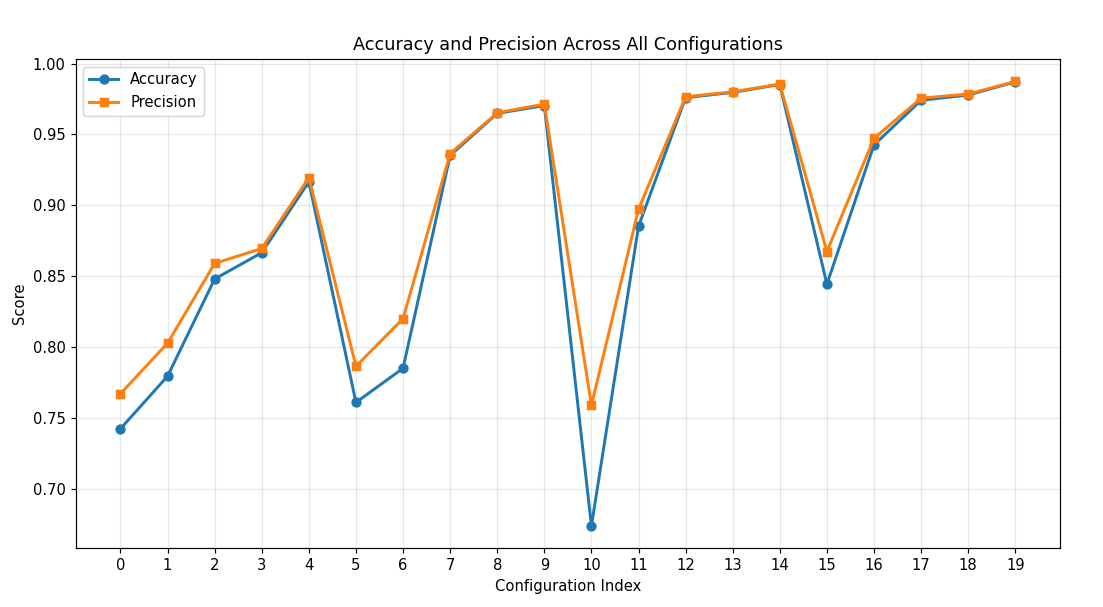
\includegraphics[width=\linewidth]{../../HMM_acc_line_validation.png}
	\caption{Accuracy και Precision κάθε διαμόρφωσης των GMM-HMM μοντέλων.\\
		Φαίνονται 4 φάσεις μήκους 5. Μεταξύ των φάσεων αυξάνεται το n\_states, ενώ εντός κάθε φάσης αυξάνεται το n\_mixtures.}
\end{figure}

\begin{figure}[H]
	\centering
	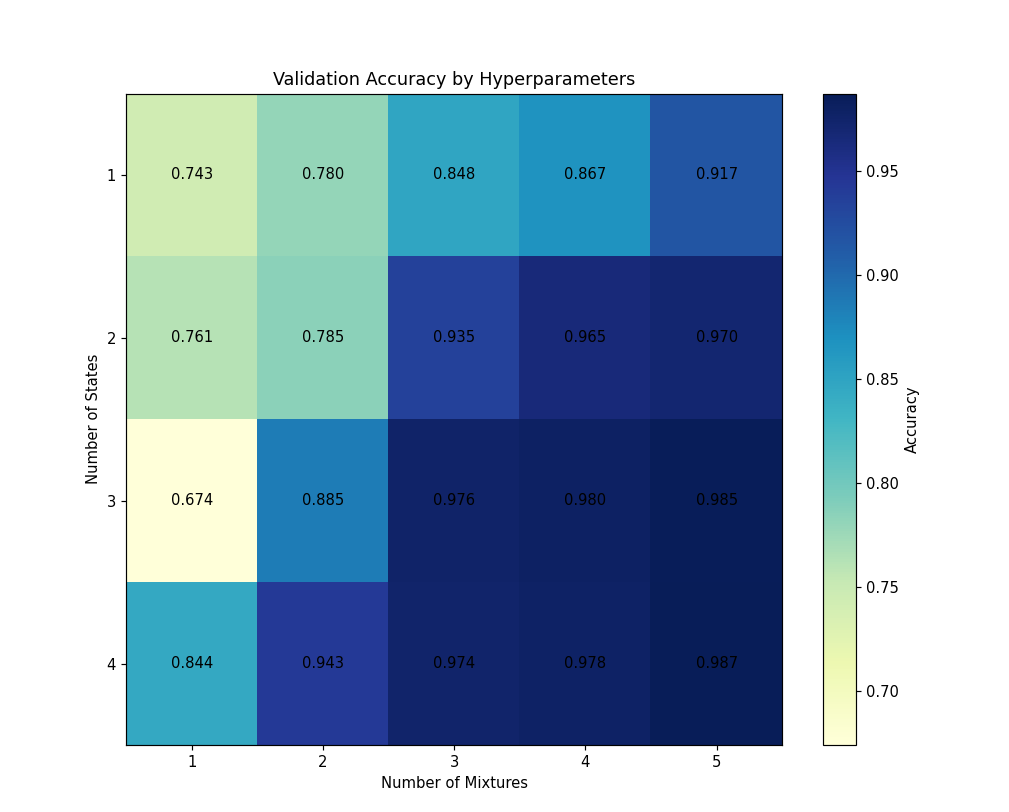
\includegraphics[width=\linewidth]{../../HMM_acc_heat_validation.png}
\end{figure}

\noindent Το καλύτερο μοντέλο είναι εμφανώς αυτό με 4 states και 5 gaussians ανά mixture και επιτυγχάνει accuracy = 98.7\% στο validation set.\\
\\
\noindent Τέλος, υπολογίζουμε την ακρίβεια του καλύτερου μοντέλου και στο testing set (ξανά καλώντας την evaluate αλλά με διαφορετικά δεδομένα). Παρατηρούμε ότι το μοντέλο έχει accuracy = 99\% στο testing set.

\begin{figure}[H]
	\centering
	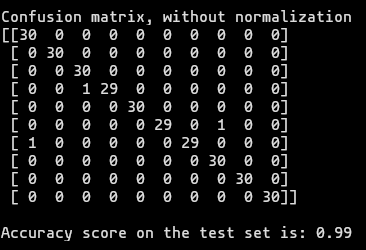
\includegraphics[width=0.5\linewidth]{../../HMM_acc_conf_testing.png}
\end{figure}

\noindent Σημειώνουμε ότι οι δοκιμές που κάνουμε στις παραμέτρους του μοντέλου, εκπαιδεύοντας μόνο στο training set θα έχουν κάποια ακρίβεια στο validation set. Με βάση μόνο αυτήν την ακρίβεια, επιλέγουμε το καλύτερο μοντέλο, και μόνο αφού έχουμε οριστικοποιήσει την επιλογή μοντέλου μας ελέγχουμε την απόδοση στο training set. Από το training set ελαχιστοποιούμε το σφάλμα εκπαίδευσης, από το validation set επιλέγουμε το καλύτερο μοντέλο, και από το testing set υπολογίζουμε εκτίμηση της ακρίβειας του μοντέλου που επιλέξαμε σε δεδομένα που δεν έχει ξαναδεί. Αυτό συμβαίνει, διότι αλλιώς, δηλαδή αν επιλέγαμε το καλύτερο μοντέλο με βάση την ακρίβεια στο training set, τότε ουσιαστικά θα εισάγαμε διαρροή δεδομένων από το testing set στο validation set, και η απόδοσή μας στο testing set δεν θα ήταν αντιπροσωπευτική της απόδοσής μας σε δεδομένα που το μοντέλο μας δεν θα είχε ξαναδεί. Το αντίστοιχο θα συνέβαινε αν χρησιμοποιούσαμε σε οποιοδήποτε σημείο προτού ολοκληρωθεί η εκπαίδευση του κάθε μοντέλο δεδομένα από το validation set. Για αυτόν τον λόγο, προσέξαμε πχ. νωρίτερα στον κώδικα να κάνουμε fit τον Scaler με βάση μόνο τα training data.




\section*{Βήμα 13}

Τέλος, υπολογίζουμε τους πίνακες σύγχυσης του καλύτερου μοντέλου στο validation και στο testing set.

\begin{figure}[H]
	\centering
	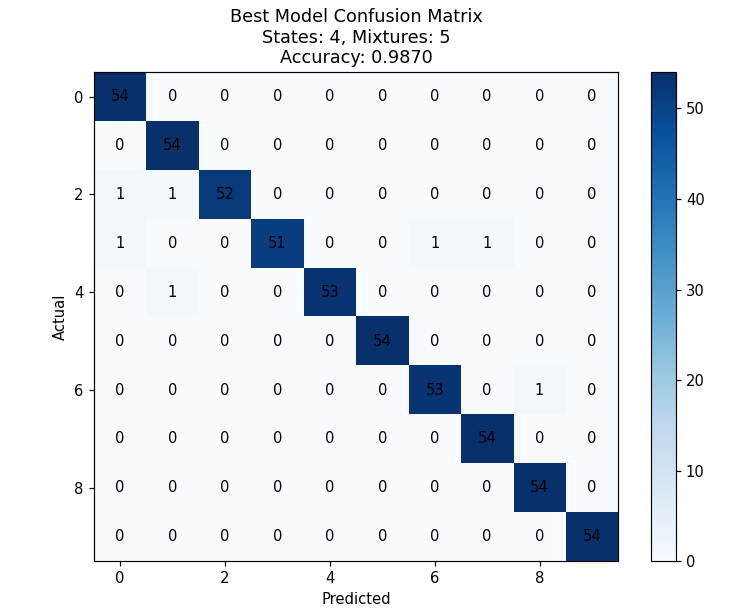
\includegraphics[width=0.8\linewidth]{../../HMM_conf_heat_validation.png}
	\caption{Πίνακας σύγχυσης του καλύτερου μοντέλου στο validation set}
\end{figure}

\begin{figure}[H]
	\centering
	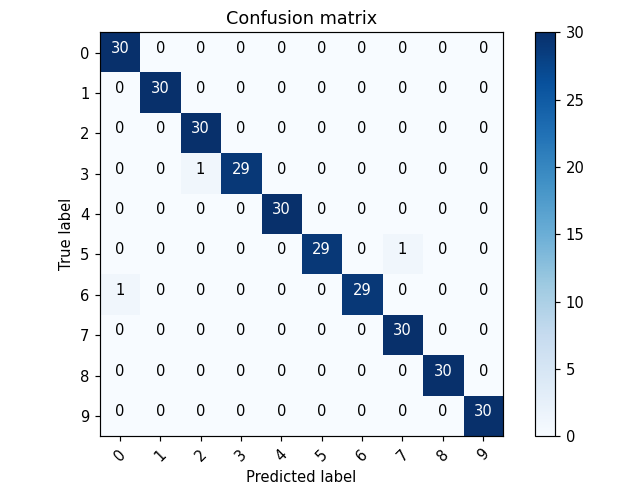
\includegraphics[width=0.8\linewidth]{../../HMM_conf_heat_testing.png}
	\caption{Πίνακας σύγχυσης στο testing set}
\end{figure}

\noindent Όπως βλέπουμε ξανά, η συνολική ακρίβεια του επιλεγμένου μοντέλου, δηλαδή το ολικό ποσοστό των σωστά κατηγοριοποιημένων εκφωνήσεων, στο testing set είναι 99\%.

\begin{figure}[H]
	\centering
	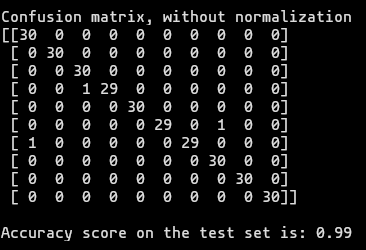
\includegraphics[width=0.5\linewidth]{../../HMM_acc_conf_testing.png}
\end{figure}

\section*{Βήμα 14}
\subsection*{1}
Η υλοποίηση του βήματος αυτού βασίζεται στη δομή του βοηθητικού κώδικα για το εργαστήριο και συγκεκριμένα στο αρχείο \textit{lstm.py}. Έχουν συμπληρωθεί τα τμήματα σημασμένα ως TODO και επιπλέον έχουν τροποποιηθεί λειτουργικότητες και προστεθεί επιπλεόν συναρτήσεις ώστε να καλυφθούν τα υποερωτήματα του βήματος.

\subsection*{2}
Για την κατασκευή του LSTM δικτύου αξιοποιήσαμε τη βιβλιοθήκη PyTorch. Ο κώδικας φαίνεται παρακάτω:

\lstinputlisting[language=Python, firstline=540, lastline=612]{../../lab.py}

\noindent Κατά την αρχικοποίηση του δικτύου ελέγχεται κατά πόσο η αρχιτεκτονική του είναι αμφίδρομη ή όχι. Εφόσον είναι, αφενός τίθεται σε True η αντίστοιχη παράμετρος και αφετέρου φροντίζουμε ώστε να διπλασιαστεί το μέγεθος του hidden state του δικτύου. \\

\noindent Στη συνέχεια, επισημαίνουμε τα είδη των layers που θα χρησιμοποιηθούν στην υλοποίηση του δικτύου. Το κυρίως layer είναι το nn.LSTM, το οποίο ρυθμίζεται με τις παραμέτρους του με τρόπο τέτοιο ώστε να καλύψει τις απαιτήσεις της εκφώνησης στα πιθανά ερωτήματα που θα προκύψουν.
\noindent Το dropout layer δεν χρησιμοποιείται πάντα. Αυτό το καθορίζουμε με την παράμετρο dropout του nn.Dropout layer. Εάν αυτή είναι 0 προφανώς αυτή η τεχνική regularization δεν χρησιμοποιείται. Επιπλέον, αξίζει να αναφέρουμε ότι έχουμε φροντίσει το Dropout να μην εφαρμοστεί στο τελευταίο layer.
\noindent Το nn.Linear layer χρησιμοποιείται ώστε να πάρει τα output του LSTM (για αυτό έχει και μέγεθος όσο του hidden state) και να τα συνδυάσει προκειμένου να πάρει την τελική απόφαση για το classification του ψηφίου. \\

\noindent Η συνάρτηση forward είναι αυτή που καθορίζει το πώς γίνεται το inference του μοντέλου. Δηλαδή, κατ' επέκταση, τη διάταξη των δομικών layers που ορίσαμε και εξηγήσαμε παραπάνω.
\noindent Ο πρώτος διαχωρισμός που κάνουμε έγκειται στο αν χρησιμοποιούμε την τεχνική packing στο input (χρειάζεται για το ερώτημα 8 - Bonus). Με την τεχνική του padding πετυχαίνουμε 2 πράγματα. Αρχικά, σε dataset με δεδομένα ακολουθίες διαφορετικών μηκών, είναι σκόπιμο να ενώσουμε τις μικρότερες από αυτές ώστε να τις επεξεργαζόμαστε ταυτόχρονα και να εξοικονομούμε χρόνο κατά την εκπαίδευση. Επιπρόσθετα, αποφεύγουμε το zero-padding και την επεξεργασία αυτής της παραμορφωμένης εκδοχής των ακολουθιών εισόδου. Η τεχνική του packing είναι ιδιαίτερα χρήσιμη σε δίκτυα στα οποία το μέγεθος εισόδου είναι αυστηρά καθορισμένο, όπως οι Transformers. 
\noindent Ο τρόπος που επιλέγουμε να εκτελέσουμε το packing είναι αρχικά να ταξινομήσουμε τις ακολουθίες με τα φωνήματα κατά φθίνον μήκος έτσι ώστε να τις συνδυάσουμε αποτελεσματικότερα. Αυτός ο συνδυασμός πραγματοποιοείται από την συνάρτηση \textit{packed\_padded\_sequence()} της βιβλιοθήκης της Pytorch (βλέπουμε ότι το enforce\_sorted είναι ορισμένο σε True). \\

\noindent Τέλος, όπως βλέπει κανείς εδώ:

\lstinputlisting[language=Python, firstline=606, lastline=610]{../../lab.py}

\lstinputlisting[language=Python, firstline=613, lastline=627]{../../lab.py}

\noindent Έτσι εξασφαλίζουμε ότι ελέγχουμε χωριστά τις ξεχωριστές ακολουθίες (με χρήση των lengths) και ότι εφαρμόζουμε το dropout πριν από το τελευταίο layer.

\subsection*{3}
Σε αυτό το βήμα καλούμαστε να εκπαιδεύσουμε το μοντέλο. Έτσι, αρχικά, θα εξηγήσουμε τη διαδικασία της εκπαίδευσής του. \\

\lstinputlisting[language=Python, firstline=668, lastline=695]{../../lab.py}

\noindent Στο training loop παίρνουμε τα δεδομένα του dataloader batch by batch, υπολογίζουμε το loss και κάνουμε το ανάλογο βήμα στον optimizer. \\

\noindent Ο optimizer που χρησιμοποιούμε είναι ο AdamW. Αξιοποιεί όρους ορμής και έχει μοντέλο για να μεταβάλει τους όρους του learning rate και της ταχύτητας κατάλληλα ώστε να επιτύχει την καλύτερη σύγκλιση. Προφανώς, εκτυπώνουμε το loss σε κάθε εποχή όπως μας ζητείται στην εκφώνηση. 

\subsection*{4}

Στην συνάρτηση train:

\lstinputlisting[language=Python, firstline=728, lastline=771]{../../lab.py}

\noindent Παίρνουμε τις μετρικές που μας ενδιαφέρουν, δηλαδή το training και validation loss καθώς και το validation accuracy. Η master train είναι αυτή που εκπαιδεύει όλα τα μοντέλα που μας ενδιαφέρουν.

\subsection*{5}
Καλούμαστε να προσθέσουμε L2 Regularization στο μοντέλο μας, καθώς και dropout. \\

\noindent Το L2 regularization δεν είναι κάτι το οποίο επηρεάζει δομικά το μοντέλο μας άμεσα. Είναι ένας όρος ποινικοποίησης του μέτρου των βαρών που προστίθεται στο loss function. Έτσι, μειώνουμε την πολυπλοκότητα του μοντέλου και έχουμε ως αποτέλεσμα την αποφυγή του overfitting. Αυτό είναι σημαντικό και αναμένεται να παίξει ρόλο, ειδικά σε ένα απλό dataset όπως είναι το δικό μας. Ένα επιπλέον πράγμα που πετυχαίνουμε είναι να αποφύγουμε το saturation στα βάρη του δικτύου μας και να ενισχύσουμε έτσι τη δυνατότητα generalization του μοντέλου μας. \\

\noindent Η τεχνική dropout απενεργοποιεί ένα ποσοστό νευρώνων (καθορίζεται από την παράμετρο dropout) κατά τη διάρκεια της εκπαίδευσης έτσι ώστε να σιγουρευτούμε ότι όλοι θα εκπαιδευτούν και έτσι θα αποφύγουμε οverfitting και το coadaptation. Προφανώς η απενεργοποίηση αυτή είναι προσωρινή και ο νευρώνας δυνητικά επανέρχεται στην επόμενη εποχή (απενεργοποιούνται άλλοι). \\

\noindent Τα χαρακτηριστικά που επιλέγουμε στην εκπαίδευση του μοντέλου μας είναι: 

\begin{itemize}
	\item epochs: 750
	\item learning rate: $2*10^{-5}$
	\item dropout: 0.4
\end{itemize}

\noindent Ο λόγος που  επιλέγουμε μικρό learning rate είναι πως κατά τη διάρκεια της εκπαίδευσης παρατηρούσαμε ταλάντωση της μετρικής accuracy για μεγαλύτερα. Έτσι, οδηγηθήκαμε και στον σχετικά μεγάλο αριθμό εποχών (750), αφού λόγω του μικρού ρυθμού μάθησης το μοντέλο αργεί να συγκλίνει. Σταματήσαμε σε αυτόν τον αριθμό διότι από εκεί και πάνω δεν παρατηρούσαμε καμία βελτίωση. 

\subsection*{6}
Αρχικά, θα εξηγήσουμε τη σημασία του early stopping και κατόπιν θα προχωρήσουμε στην ανάλυση της δικής μας υλοποίησης. \\

\noindent Με το early stopping διακόπτουμε πρόωρα την εκπαίδευση του μοντέλου (πριν τη συμπλήρωση του προαπαιτούμενου αριθμού εποχών). Αυτό γίνεται με αυτόματο τρόπο. Ουσιαστικά, αν συμπληρωθεί ένας ορισμένος αριθμός εποχών (εδώ patience είναι 10) στον οποίο το μοντέλο μας δεν βελτιώνεται, σταματάμε. Με αυτό τον τρόπο πετυχαίνουμε τα εξής:

\begin{itemize}
	\item Αποτρέπει το overfitting 
	
	\item  Εξοικονομεί χρόνο και πόρους. Αν το μοντέλο έχει πρακτικά συγκλίνει σε μικρότερο αριθμό εποχών από αυτόν που αναμένουμε, δεν συνεχίζουμε άσκοπα.
\end{itemize}

\noindent Στον κώδικά μας χρησιμοποιούμε την κλάση EarlyStopping:

\lstinputlisting[language=Python, firstline=467, lastline=500]{../../lab.py}

\noindent Κεντρική μέθοδός της είναι η stop. Ουσιαστικά ελέγχει κατά πόσο έχει βελτιωθεί το μοντέλο μας σε σχέση με την προηγούμενη εποχή (το συγκρίνει με το μέχρι τώρα καλύτερο) και, εφόσον δεν έχει βελτιωθεί, αφαιρεί μία εποχή από το περιθώριο υπομονής μας (\textit{patience\_left}). Όταν αυτό εξαντληθεί, δηλαδή φτάσει στο 0, αποθηκεύουμε το μοντέλο μας σε pickle format με τις κατάλληλες συναρτήσεις της PyTorch.

\subsection*{7}
Σε αυτό το υποερώτημα καλούμαστε να πειραματιστούμε και με ένα bidirectional LSTM. Όπως έχουμε εξηγήσει παραπάνω, ο τρόπος ώστε το μοντέλο μας να γίνεται αμφίδρομο είναι να θέσουμε True την κατάλληλη παράμετρο και οι κατάλληλες προσαρμογές γίνονται αυτόματα από τον κώδικά μας για το μοντέλο.\\

\noindent Ουστιαστικά, το bidirectional LSTM έχει τα διπλάσια κύτταρα LSTM από το απλό. Τα μισά διαδίδουν πληροφορία του hidden state προς τα εμπρός, όπως και πριν, ενώ τα άλλα μισά κάνουν το ίδιο αλλά στην αντίστροφη κατεύθυνση. \\

\noindent Η ανάγνωση της ακολουθίας εισόδου τόσο από την αρχή προς το τέλος της όσο και αντίστροφα, μας επιτρέπει να καταλάβουμε το context και τα συμφραζόμενα καλύτερα. Προφανώς, αυτό ισχύει και έχει σημασία και στην προφορά των ψηφίων αφού για παράδειγμα τόσο το two όσο και το three ξεκινούν με το ίδιο σύμφωνο ήχο ενώ τελειώνουν με διαφορετικό. Επίσης, με τα αμφίδρομα LSTM μπορούμε να αντιμετωπίσουμε καλύτερα την "απώλεια μνήμης" για μεγάλες ακολουθίες. Προφανώς όταν μία ακολουθία είναι μεγάλη, το context και η πληροφορία της αρχής ξεθωριάζει καθώς ξεδιπλώνουμε το LSTM. Τώρα, όμως, διαβάζοντάς τη και από το τέλος έχουμε καλύτερη συγκράτηση και συνδυασμό πληροφορίας από όλο το μήκος της ακολουθίας. Η αύξηση αυτή της χωρητικότητας του μοντέλου που περιγράφουμε οδηγεί συνήθως και σε αύξηση της απόδοσής του.

\subsection*{8}
Στο τελευταίο Bonus υποερώτημα καλούμαστε να πειραματιστούμε με την τεχνική του packing. Ο τρόπος με τον οποίο λειτουργεί εξηγήθηκε στο υποερώτημα 2. Συνοψίζουμε τα πλεονεκτήματά του:

\begin{itemize}
	\item Αποφυγή θορύβου από το padding στο dataset
	
	\item Αύξηση της ταχύτητας εκπαίδευσης αφού βλέπουμε πολλές μικρές ακολουθίες ταυτόχρονα αντί ξεχωριστά
	
	\item Βελτίωση της αριθμητικής ευρωστείας του μοντέλου, αφού όλο και λιγότερα δείγματα (συνεχόμενα κιόλας) είναι μηδενικά και έτσι τα gradients είναι "καθαρότερα"
\end{itemize}

\subsection*{Αποτελέσματα}
Μετά την περιήγηση στα υποερωτήματα μας θα παρουσιάσουμε τα αποτελέσματα των πειραματισμών μας. 

\begin{figure}[H]
	\centering
	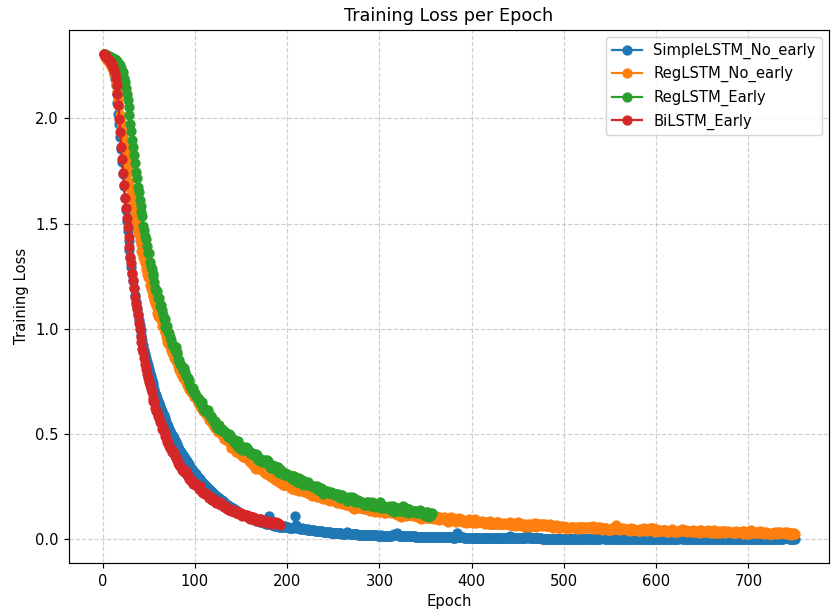
\includegraphics[width=0.75\linewidth]{images/lstm_train_loss.png}
	\caption{Models' Train Loss}
\end{figure}

\noindent Το να παραθέσουμε τα prints του training loss σε κάθε εποχή μπορεί να βοήθησε στο tuning των epochs και του learning rate αλλά δεν έχει νόημα να τα παρουσιάσουμε με λεπτομέρεια στην αναφορά. Αντί αυτού έχουμε κάνει το παραπάνω plot που απεικονίζει τη σύγκλιση όλων των μοντέλων που εκπαιδεύσαμε. \\

\noindent Όπως παρατηρούμε στο διάγραμμα, το early stopping πράγματι λειτουργεί διακόπτοντας την εκπαίδευση των μοντέλων που το χρησιμοποιούν όταν αυτά έχουν σχεδόν σταθεροποιηθεί. Αυτό γλιτώνει πάνω από το μισό χρόνο εκπαίδευσης δίχως να έχει μεγάλη επίπτωση στην απόδοση - όπως θα δούμε σε λίγο. Επίσης, όπως είναι λογικό, τα μοντέλα που χρησιμοποιούν regularization γενικά συγκλίνουν πιο αργά. Αυτό συμβαίνει αφενός λόγω του dropout το οποίο απενεργοποιεί διάφορους νευρώνες καθιστώντας πιο αργή την individual σύγκλισή τους και αφετέρου επειδή το L2 regularization δεν ευνοεί επίσης την ταχύτητα σύγκλισης. Το Bidirectional LSTM χρησιμοποιεί και αυτό regularization αλλά συγκλίνει πολύ γρήγορα λόγω της ευκρίνειας στα gradients που δίνεται από την πιο πλούσια πληροφορία.

\begin{figure}[H]
	\centering
	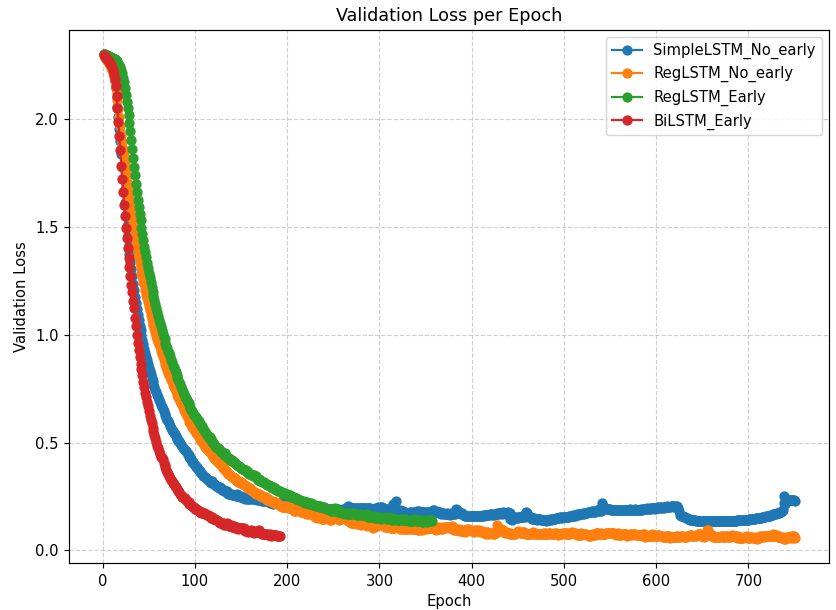
\includegraphics[width=0.75\linewidth]{images/lstm_va_loss.png}
	\caption{Models' Validation Loss}
\end{figure}

\noindent Γενικά, ένα μοντέλο στο οποίο δεν υπάρχει overfitting, πρέπει να έχει παρόμοια εξέλιξη στην σύγκλιση του validation και του trainning accuracy και πιο σημαντικά, στην κατάσταση σύγκλισης να μην υπάρχει χάσμα μεταξύ στις δύο μετρικές (προφανώς δεν μπορεί ποτέ να έχουμε καλύτερο accuracy στο validation set από ότι στο train αλλά πρέπει να είναι κοντά). Όπως βλέπουμε στο διάγραμμα, στο μόνο μοντέλο στο οποίο αυτό δεν συμβαίνει, δηλαδή βλέπουμε δείγματα overfitting είναι στο απλό μοντέλο δίχως χρήση regularization. Αυτό είναι απολύτως λογικό, αφού η χωρητικότητα του μοντέλου υπερκαλύπτει τις ανάγκες του task και δεν υπάρχει κανένας μηχανισμός αποφυγής της υπερπροσαρμογής του στα δεδομένα εκπαίδευσης. Αυτό δεν συμβαίνει με τα υπόλοιπα μοντέλα που χρησιμοποιείται regularization πράγμα που επιβεβαιώνει την αποτελεσματικότητά του και τη σωστή χρήση του στον κώδικά μας.

\begin{figure}[H]
	\centering
	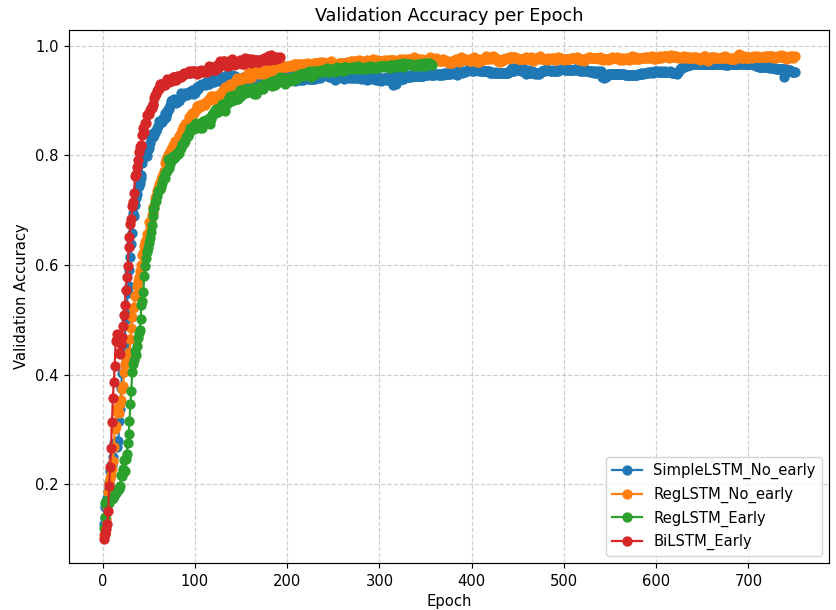
\includegraphics[width=0.7\linewidth]{images/lstm_val_acc.png}
	\caption{Models' Validation Accuracy}
\end{figure}

\noindent Όπως είναι λογικό, το accuracy στο validation set ακολουθεί αντίστροφη πορεία σύγκλισης από το loss σε όλα τα μοντέλα.

\begin{figure}[H]
	\centering
	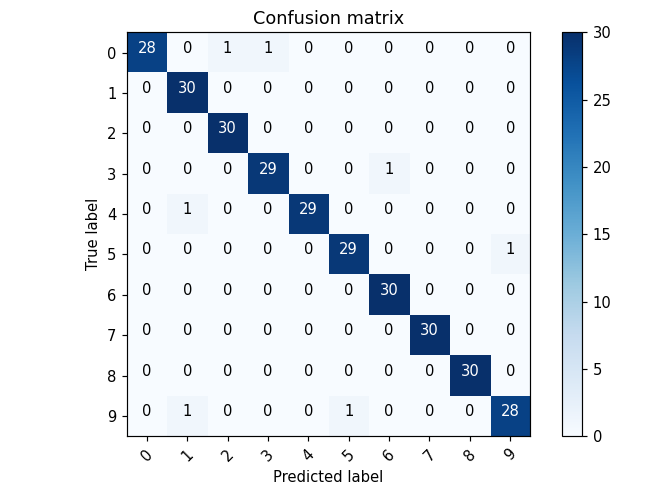
\includegraphics[width=0.7\linewidth]{images/test_cm_lstm.png}
	\caption{Confusion Matrix}
\end{figure}

\noindent Το confusion matrix στο test set δείχνει πως το καλύτερο μοντέλο μας τα πάει εξαιρετικά αφού κάνει ελάχιστα λάθη σε όλα τα ψηφία.

\begin{figure}[H]
	\centering
	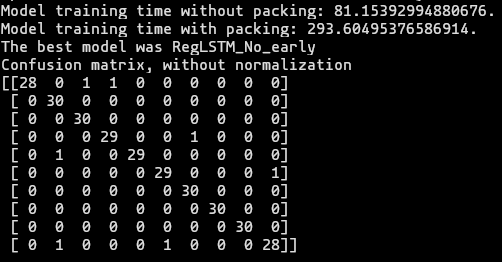
\includegraphics[width=0.7\linewidth]{images/result_lstm_packing.png}
	\caption{Confusion Matrix}
\end{figure}

\noindent Το καλύτερο μοντέλο από άποψη βέλτιστου accuracy στο validation dataset είναι το LSTM στο οποίο έχουν χρησιμοποιηθεί τεχνικές regularization. Το test accuracy του είναι 97.7\%. 

\noindent Για το bonus ερώτημα βλέπουμε κάτι παράδοξο. Ενώ περιμέναμε το packing να είναι γρηγορότερο από το μη packing συμβαίνει το αντίθετο! Αυτό γίνεται διότι για να ταξινομήσουμε τις ακολουθίες κατά φθίνουσα σειρά μήκους πρέπει να φέρουμε τα μήκη στη cpu από τη gpu του υπολογιστή που εκπαιδεύαμε τα μοντέλα. Για τόσο μικρό dataset το χρονικό overhead αυτής της μεταφοράς δεδομένων είναι σημαντικά μεγαλύτερο του χρόνου που θα χρειαζόταν οι πράξεις για την εκπαίδευση κάποιων περισσότερων ακολουθιών με zero-padding.  \\

\noindent Ακολουθεί το διάγραμμα με το training και validation loss για το καλύτερό μας μοντέλο:

\begin{figure}[H]
	\centering
	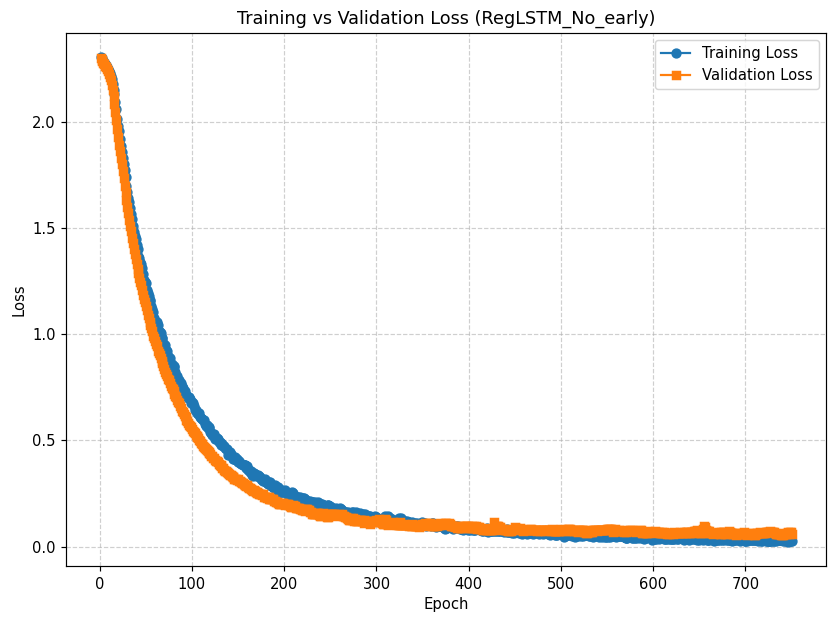
\includegraphics[width=0.7\linewidth]{images/best_train_val.png}
	\caption{Confusion Matrix}
\end{figure}





\bibliographystyle{plain}
\bibliography{bibliography}

\end{document}